\documentclass[aspectratio=169]{beamer}

%\documentclass[handout]{beamer}
%% To make 4 per page
%\usepackage{pgfpages}
%\mode<handout>{\setbeamercolor{background canvas}{bg=white}}
%\pgfpagesuselayout{4 on 1}[letterpaper,landscape]%,border shrink=5mm]

\usetheme{default}
% Slide setup, colour independent

\usepackage{amsmath,amssymb,amsthm}
\usepackage{colortbl}
\usepackage{bm}
\usepackage{xcolor}
\usepackage{dsfont}
\usepackage{setspace}
%\usepackage{subfigure}
% To use \ding{234} and the like
\usepackage{pifont}
% To cross reference between slide files
\usepackage{zref-xr,zref-user}
% Use something like
% \zexternaldocument{fileI}
% in the tex files. And cite using \zref instead of \ref

% Fields and the like
\def\IC{\mathbb{C}}
\def\IF{\mathbb{F}}
\def\II{\mathbb{I}}
\def\IJ{\mathbb{J}}
\def\IM{\mathbb{M}}
\def\IN{\mathbb{N}}
\def\IP{\mathbb{P}}
\def\IR{\mathbb{R}}
\def\IZ{\mathbb{Z}}
\def\11{\mathds{1}}


% Bold lowercase
\def\ba{\mathbf{a}}
\def\bb{\mathbf{b}}
\def\bc{\mathbf{c}}
\def\bd{\mathbf{d}}
\def\be{\mathbf{e}}
\def\bf{\mathbf{f}}
\def\bh{\mathbf{h}}
\def\bi{\mathbf{i}}
\def\bj{\mathbf{j}}
\def\bk{\mathbf{k}}
\def\bn{\mathbf{n}}
\def\bp{\mathbf{p}}
\def\br{\mathbf{r}}
\def\bs{\mathbf{s}}
\def\bu{\mathbf{u}}
\def\bv{\mathbf{v}}
\def\bw{\mathbf{w}}
\def\bx{\mathbf{x}}
\def\by{\mathbf{y}}
\def\bz{\mathbf{z}}

% Bold capitals
\def\bB{\mathbf{B}}
\def\bD{\mathbf{D}}
\def\bF{\mathbf{F}}
\def\bG{\mathbf{G}}
\def\bI{\mathbf{I}}
\def\bL{\mathbf{L}}
\def\bN{\mathbf{N}}
\def\bP{\mathbf{P}}
\def\bR{\mathbf{R}}
\def\bS{\mathbf{S}}
\def\bT{\mathbf{T}}
\def\bX{\mathbf{X}}

% Bold numbers
\def\b0{\mathbf{0}}

% Bold greek
\bmdefine{\bmu}{\bm{\mu}}
\def\bphi{\bm{\phi}}
\def\bvarphi{\bm{\varphi}}

% Bold red sentence
\def\boldred#1{{\color{red}\textbf{#1}}}
\def\defword#1{{\color{orange}\textbf{#1}}}

% Caligraphic letters
\def\A{\mathcal{A}}
\def\B{\mathcal{B}}
\def\C{\mathcal{C}}
\def\D{\mathcal{D}}
\def\E{\mathcal{E}}
\def\F{\mathcal{F}}
\def\G{\mathcal{G}}
\def\H{\mathcal{H}}
\def\I{\mathcal{I}}
\def\L{\mathcal{L}}
\def\M{\mathcal{M}}
\def\N{\mathcal{N}}
\def\P{\mathcal{P}}
\def\R{\mathcal{R}}
\def\S{\mathcal{S}}
\def\T{\mathcal{T}}
\def\U{\mathcal{U}}
\def\V{\mathcal{V}}

% tt font for code
\def\code#1{{\tt #1}}

% i.e., e.g.
\def\eg{\emph{e.g.}}
\def\ie{\emph{i.e.}}


% Operators and special symbols
\def\nbOne{{\mathchoice {\rm 1\mskip-4mu l} {\rm 1\mskip-4mu l}
{\rm 1\mskip-4.5mu l} {\rm 1\mskip-5mu l}}}
\def\cov{\ensuremath{\mathsf{cov}}}
\def\Var{\ensuremath{\mathsf{Var}\ }}
\def\Im{\textrm{Im}\;}
\def\Re{\textrm{Re}\;}
\def\det{\ensuremath{\mathsf{det}}}
\def\diag{\ensuremath{\mathsf{diag}}}
\def\nullspace{\ensuremath{\mathsf{null}}}
\def\nullity{\ensuremath{\mathsf{nullity}}}
\def\rank{\ensuremath{\mathsf{rank}}}
\def\range{\ensuremath{\mathsf{range}}}
\def\sgn{\ensuremath{\mathsf{sgn}}}
\def\Span{\ensuremath{\mathsf{span}}}
\def\tr{\ensuremath{\mathsf{tr}}}
\def\imply{$\Rightarrow$}
\def\restrictTo#1#2{\left.#1\right|_{#2}}
\newcommand{\parallelsum}{\mathbin{\!/\mkern-5mu/\!}}
\def\dsum{\mathop{\displaystyle \sum }}%
\def\dind#1#2{_{\substack{#1\\ #2}}}

\DeclareMathOperator{\GL}{GL}
\DeclareMathOperator{\Rel}{Re}
\def\Nt#1{\left|\!\left|\!\left|#1\right|\!\right|\!\right|}
\newcommand{\tripbar}{|\! |\! |}



% The beamer bullet (in base colour)
\def\bbullet{\leavevmode\usebeamertemplate{itemize item}\ }

% Theorems and the like
\newtheorem{proposition}[theorem]{Proposition}
\newtheorem{property}[theorem]{Property}
\newtheorem{importantproperty}[theorem]{Property}
\newtheorem{importanttheorem}[theorem]{Theorem}
%\newtheorem{lemma}[theorem]{Lemma}
%\newtheorem{corollary}[theorem]{Corollary}
\newtheorem{remark}[theorem]{Remark}
\setbeamertemplate{theorems}[numbered]
%\setbeamertemplate{theorems}[ams style]

%
%\usecolortheme{orchid}
%\usecolortheme{orchid}

\def\red{\color[rgb]{1,0,0}}
\def\blue{\color[rgb]{0,0,1}}
\def\green{\color[rgb]{0,1,0}}


% Get rid of navigation stuff
\setbeamertemplate{navigation symbols}{}

% Set footline/header line
\setbeamertemplate{footline}
{%
\quad p. \insertpagenumber \quad--\quad \insertsection\vskip2pt
}
% \setbeamertemplate{headline}
% {%
% \quad\insertsection\hfill p. \insertpagenumber\quad\mbox{}\vskip2pt
% }


\makeatletter
\newlength\beamerleftmargin
\setlength\beamerleftmargin{\Gm@lmargin}
\makeatother

% Colours for special pages
\def\extraContent{yellow!20}


%%%%%%%%%%%%%%%%%
\usepackage{tikz}
\usetikzlibrary{shapes,arrows}
\usetikzlibrary{positioning}
\usetikzlibrary{shapes.symbols,shapes.callouts,patterns}
\usetikzlibrary{calc,fit}
\usetikzlibrary{backgrounds}
\usetikzlibrary{decorations.pathmorphing,fit,petri}
\usetikzlibrary{automata}
\usetikzlibrary{fadings}
\usetikzlibrary{patterns,hobby}

\usetikzlibrary{backgrounds,fit,petri}


\usepackage{pgfplots}
\pgfplotsset{compat=1.6}
\pgfplotsset{ticks=none}

\usetikzlibrary{decorations.markings}
\usetikzlibrary{arrows.meta}
\tikzset{>=stealth}

% For tikz
\usetikzlibrary{shapes,arrows}
\usetikzlibrary{positioning}
\tikzstyle{cloud} = [draw, ellipse,fill=red!20, node distance=0.87cm,
minimum height=2em]
\tikzstyle{line} = [draw, -latex']


%%% For max frame images
\newenvironment{changemargin}[2]{%
\begin{list}{}{%
\setlength{\topsep}{0pt}%
\setlength{\leftmargin}{#1}%
\setlength{\rightmargin}{#2}%
\setlength{\listparindent}{\parindent}%
\setlength{\itemindent}{\parindent}%
\setlength{\parsep}{\parskip}%
}%
\item[]}{\end{list}}


% Make one image take up the entire slide content area in beamer,.:
% centered/centred full-screen image, with title:
% This uses the whole screen except for the 1cm border around it
% all. 128x96mm
\newcommand{\titledFrameImage}[2]{
\begin{frame}{#1}
%\begin{changemargin}{-1cm}{-1cm}
\begin{center}
\includegraphics[width=108mm,height=\textheight,keepaspectratio]{#2}
\end{center}
%\end{changemargin}
\end{frame}
}

% Make one image take up the entire slide content area in beamer.:
% centered/centred full-screen image, no title:
% This uses the whole screen except for the 1cm border around it
% all. 128x96mm
\newcommand{\plainFrameImage}[1]{
\begin{frame}[plain]
%\begin{changemargin}{-1cm}{-1cm}
\begin{center}
\includegraphics[width=108mm,height=76mm,keepaspectratio]{#1}
\end{center}
%\end{changemargin}
\end{frame}
}

% Make one image take up the entire slide area, including borders, in beamer.:
% centered/centred full-screen image, no title:
% This uses the entire whole screen
\newcommand{\maxFrameImage}[1]{
\begin{frame}[plain]
\begin{changemargin}{-1cm}{-1cm}
\begin{center}
\includegraphics[width=\paperwidth,height=\paperheight,keepaspectratio]
{#1}
\end{center}
\end{changemargin}
\end{frame}
}

% This uses the entire whole screen (to include in frame)
\newcommand{\maxFrameImageNoFrame}[1]{
\begin{changemargin}{-1cm}{-1cm}
\begin{center}
\includegraphics[width=\paperwidth,height=0.99\paperheight,keepaspectratio]
{#1}
\end{center}
\end{changemargin}
}

% Make one image take up the entire slide area, including borders, in beamer.:
% centered/centred full-screen image, no title:
% This uses the entire whole screen
\newcommand{\maxFrameImageColor}[2]{
\begin{frame}[plain]
\setbeamercolor{normal text}{bg=#2!20}
\begin{changemargin}{-1cm}{-1cm}
\begin{center}
\includegraphics[width=\paperwidth,height=\paperheight,keepaspectratio]
{#1}
\end{center}
\end{changemargin}
\end{frame}
}


\usepackage{tikz}
\usetikzlibrary{patterns,hobby}
\usepackage{pgfplots}
\pgfplotsset{compat=1.6}
\pgfplotsset{ticks=none}

\usetikzlibrary{backgrounds}
\usetikzlibrary{decorations.markings}
\usetikzlibrary{arrows.meta}
\tikzset{>=stealth}

\tikzset{
  clockwise arrows/.style={
    postaction={
      decorate,
      decoration={
        markings,
        mark=between positions 0.1 and 0.9 step 40pt with {\arrow{>}},
   }}}}


   %%%%%%%%%%%
% To have links to parts in the outline
\makeatletter
\AtBeginPart{%
  \addtocontents{toc}{\protect\beamer@partintoc{\the\c@part}{\beamer@partnameshort}{\the\c@page}}%
}
%% number, shortname, page.
\providecommand\beamer@partintoc[3]{%
  \ifnum\c@tocdepth=-1\relax
    % requesting onlyparts.
    \makebox[6em]{Part #1:} \textcolor{green!30!blue}{\hyperlink{#2}{#2}}
    \par
  \fi
}
\define@key{beamertoc}{onlyparts}[]{%
  \c@tocdepth=-1\relax
}
\makeatother%

\newcommand{\nameofthepart}{}
\newcommand{\nupart}[1]%
    {   \part{#1}%
        \renewcommand{\nameofthepart}{#1}%
        {
          \setbeamercolor{background canvas}{bg=orange!50}
          \begin{frame}{#1}%\partpage 
          \hypertarget{\nameofthepart}{}\tableofcontents%
          \end{frame}
        }
    }



\usecolortheme{orchid}

%% Listings
\usepackage{listings}
\definecolor{mygreen}{rgb}{0,0.6,0}
\definecolor{mygray}{rgb}{0.5,0.5,0.5}
\definecolor{mymauve}{rgb}{0.58,0,0.82}
\definecolor{mygold}{rgb}{1,0.843,0}
\definecolor{myblue}{rgb}{0.537,0.812,0.941}

\definecolor{lgreen}{rgb}{0.6,0.9,.6}
\definecolor{lred}{rgb}{1,0.5,.5}

\lstloadlanguages{R}
\lstset{ %
  language=R,
  backgroundcolor=\color{black!05},   % choose the background color
  basicstyle=\footnotesize\ttfamily,        % size of fonts used for the code
  breaklines=true,                 % automatic line breaking only at whitespace
  captionpos=b,                    % sets the caption-position to bottom
  commentstyle=\color{mygreen},    % comment style
  escapeinside={\%*}{*)},          % if you want to add LaTeX within your code
  keywordstyle=\color{red},       % keyword style
  stringstyle=\color{mygold},     % string literal style
  keepspaces=true,
  columns=fullflexible,
  tabsize=4,
}
% Could also do (in lstset)
% basicstyle==\fontfamily{pcr}\footnotesize
\lstdefinelanguage{Renhanced}%
  {keywords={abbreviate,abline,abs,acos,acosh,action,add1,add,%
      aggregate,alias,Alias,alist,all,anova,any,aov,aperm,append,apply,%
      approx,approxfun,apropos,Arg,args,array,arrows,as,asin,asinh,%
      atan,atan2,atanh,attach,attr,attributes,autoload,autoloader,ave,%
      axis,backsolve,barplot,basename,besselI,besselJ,besselK,besselY,%
      beta,binomial,body,box,boxplot,break,browser,bug,builtins,bxp,by,%
      c,C,call,Call,case,cat,category,cbind,ceiling,character,char,%
      charmatch,check,chol,chol2inv,choose,chull,class,close,cm,codes,%
      coef,coefficients,co,col,colnames,colors,colours,commandArgs,%
      comment,complete,complex,conflicts,Conj,contents,contour,%
      contrasts,contr,control,helmert,contrib,convolve,cooks,coords,%
      distance,coplot,cor,cos,cosh,count,fields,cov,covratio,wt,CRAN,%
      create,crossprod,cummax,cummin,cumprod,cumsum,curve,cut,cycle,D,%
      data,dataentry,date,dbeta,dbinom,dcauchy,dchisq,de,debug,%
      debugger,Defunct,default,delay,delete,deltat,demo,de,density,%
      deparse,dependencies,Deprecated,deriv,description,detach,%
      dev2bitmap,dev,cur,deviance,off,prev,,dexp,df,dfbetas,dffits,%
      dgamma,dgeom,dget,dhyper,diag,diff,digamma,dim,dimnames,dir,%
      dirname,dlnorm,dlogis,dnbinom,dnchisq,dnorm,do,dotplot,double,%
      download,dpois,dput,drop,drop1,dsignrank,dt,dummy,dump,dunif,%
      duplicated,dweibull,dwilcox,dyn,edit,eff,effects,eigen,else,%
      emacs,end,environment,env,erase,eval,equal,evalq,example,exists,%
      exit,exp,expand,expression,External,extract,extractAIC,factor,%
      fail,family,fft,file,filled,find,fitted,fivenum,fix,floor,for,%
      For,formals,format,formatC,formula,Fortran,forwardsolve,frame,%
      frequency,ftable,ftable2table,function,gamma,Gamma,gammaCody,%
      gaussian,gc,gcinfo,gctorture,get,getenv,geterrmessage,getOption,%
      getwd,gl,glm,globalenv,gnome,GNOME,graphics,gray,grep,grey,grid,%
      gsub,hasTsp,hat,heat,help,hist,home,hsv,httpclient,I,identify,if,%
      ifelse,Im,image,\%in\%,index,influence,measures,inherits,install,%
      installed,integer,interaction,interactive,Internal,intersect,%
      inverse,invisible,IQR,is,jitter,kappa,kronecker,labels,lapply,%
      layout,lbeta,lchoose,lcm,legend,length,levels,lgamma,library,%
      licence,license,lines,list,lm,load,local,locator,log,log10,log1p,%
      log2,logical,loglin,lower,lowess,ls,lsfit,lsf,ls,machine,Machine,%
      mad,mahalanobis,make,link,margin,match,Math,matlines,mat,matplot,%
      matpoints,matrix,max,mean,median,memory,menu,merge,methods,min,%
      missing,Mod,mode,model,response,mosaicplot,mtext,mvfft,na,nan,%
      names,omit,nargs,nchar,ncol,NCOL,new,next,NextMethod,nextn,%
      nlevels,nlm,noquote,NotYetImplemented,NotYetUsed,nrow,NROW,null,%
      numeric,\%o\%,objects,offset,old,on,Ops,optim,optimise,optimize,%
      options,or,order,ordered,outer,package,packages,page,pairlist,%
      pairs,palette,panel,par,parent,parse,paste,path,pbeta,pbinom,%
      pcauchy,pchisq,pentagamma,persp,pexp,pf,pgamma,pgeom,phyper,pico,%
      pictex,piechart,Platform,plnorm,plogis,plot,pmatch,pmax,pmin,%
      pnbinom,pnchisq,pnorm,points,poisson,poly,polygon,polyroot,pos,%
      postscript,power,ppoints,ppois,predict,preplot,pretty,Primitive,%
      print,prmatrix,proc,prod,profile,proj,prompt,prop,provide,%
      psignrank,ps,pt,ptukey,punif,pweibull,pwilcox,q,qbeta,qbinom,%
      qcauchy,qchisq,qexp,qf,qgamma,qgeom,qhyper,qlnorm,qlogis,qnbinom,%
      qnchisq,qnorm,qpois,qqline,qqnorm,qqplot,qr,Q,qty,qy,qsignrank,%
      qt,qtukey,quantile,quasi,quit,qunif,quote,qweibull,qwilcox,%
      rainbow,range,rank,rbeta,rbind,rbinom,rcauchy,rchisq,Re,read,csv,%
      csv2,fwf,readline,socket,real,Recall,rect,reformulate,regexpr,%
      relevel,remove,rep,repeat,replace,replications,report,require,%
      resid,residuals,restart,return,rev,rexp,rf,rgamma,rgb,rgeom,R,%
      rhyper,rle,rlnorm,rlogis,rm,rnbinom,RNGkind,rnorm,round,row,%
      rownames,rowsum,rpois,rsignrank,rstandard,rstudent,rt,rug,runif,%
      rweibull,rwilcox,sample,sapply,save,scale,scan,scan,screen,sd,se,%
      search,searchpaths,segments,seq,sequence,setdiff,setequal,set,%
      setwd,show,sign,signif,sin,single,sinh,sink,solve,sort,source,%
      spline,splinefun,split,sqrt,stars,start,stat,stem,step,stop,%
      storage,strstrheight,stripplot,strsplit,structure,strwidth,sub,%
      subset,substitute,substr,substring,sum,summary,sunflowerplot,svd,%
      sweep,switch,symbol,symbols,symnum,sys,status,system,t,table,%
      tabulate,tan,tanh,tapply,tempfile,terms,terrain,tetragamma,text,%
      time,title,topo,trace,traceback,transform,tri,trigamma,trunc,try,%
      ts,tsp,typeof,unclass,undebug,undoc,union,unique,uniroot,unix,%
      unlink,unlist,unname,untrace,update,upper,url,UseMethod,var,%
      variable,vector,Version,vi,warning,warnings,weighted,weights,%
      which,while,window,write,\%x\%,x11,X11,xedit,xemacs,xinch,xor,%
      xpdrows,xy,xyinch,yinch,zapsmall,zip},%
   otherkeywords={!,!=,~,$,*,\%,\&,\%/\%,\%*\%,\%\%,<-,<<-,_,/},%
   alsoother={._$},%
   sensitive,%
   morecomment=[l]\#,%
   morestring=[d]",%
   morestring=[d]'% 2001 Robert Denham
  }%

%%%%%%% 
%% Definitions in yellow boxes
\usepackage{etoolbox}
\setbeamercolor{block title}{use=structure,fg=structure.fg,bg=structure.fg!40!bg}
\setbeamercolor{block body}{parent=normal text,use=block title,bg=block title.bg!20!bg}

\BeforeBeginEnvironment{definition}{%
	\setbeamercolor{block title}{fg=black,bg=yellow!20!white}
	\setbeamercolor{block body}{fg=black, bg=yellow!05!white}
}
\AfterEndEnvironment{definition}{
	\setbeamercolor{block title}{use=structure,fg=structure.fg,bg=structure.fg!20!bg}
	\setbeamercolor{block body}{parent=normal text,use=block title,bg=block title.bg!50!bg, fg=black}
}
\BeforeBeginEnvironment{importanttheorem}{%
	\setbeamercolor{block title}{fg=black,bg=red!20!white}
	\setbeamercolor{block body}{fg=black, bg=red!05!white}
}
\AfterEndEnvironment{importanttheorem}{
	\setbeamercolor{block title}{use=structure,fg=structure.fg,bg=structure.fg!20!bg}
	\setbeamercolor{block body}{parent=normal text,use=block title,bg=block title.bg!50!bg, fg=black}
}
\BeforeBeginEnvironment{importantproperty}{%
	\setbeamercolor{block title}{fg=black,bg=red!50!white}
	\setbeamercolor{block body}{fg=black, bg=red!30!white}
}
\AfterEndEnvironment{importantproperty}{
	\setbeamercolor{block title}{use=structure,fg=structure.fg,bg=structure.fg!20!bg}
	\setbeamercolor{block body}{parent=normal text,use=block title,bg=block title.bg!50!bg, fg=black}
}


% Beginning of a section
\AtBeginSection[]{
	{
		\setbeamercolor{background canvas}{bg=yellow!10}
		\begin{frame}[noframenumbering,plain]
			\framesubtitle{\nameofthepart Chapter \insertromanpartnumber \ -- \iteminsert{\insertpart}}
			\tableofcontents[
				currentsection,
				sectionstyle=show/shaded,
				subsectionstyle=show/show/hide]
		\end{frame}
	\addtocounter{page}{-1}
	%\addtocounter{framenumber}{-1} 
	}
}

% Beginning of a section
\AtBeginSubsection[]{
	{
		\setbeamercolor{background canvas}{bg=green!10}
		\begin{frame}[noframenumbering,plain]
				\framesubtitle{\nameofthepart Chapter \insertromanpartnumber \ -- \iteminsert{\insertpart}}
				\tableofcontents[
					currentsection,
					sectionstyle=show/show,
					currentsubsection,
					subsectionstyle=show/shaded/hide]
			\end{frame}
		\addtocounter{page}{-1}
	}
}




\title{Quick review of 2nd year linear algebra}
\author{Julien Arino}
\date{Fall 2023}

%%%%%%%%%%%%%%%%%%%%%
%%%%%%%%%%%%%%%%%%%%%
%%%%%%%%%%%%%%%%%%%%%
%%%%%%%%%%%%%%%%%%%%%
%%%%%%%%%%%%%%%%%%%%%
%%%%%%%%%%%%%%%%%%%%%
%%%%%%%%%%%%%%%%%%%%%
%%%%%%%%%%%%%%%%%%%%%
\begin{document}

% The title page
\begin{frame}[noframenumbering,plain]
    \begin{tikzpicture}[remember picture,overlay]
        \node[above right,inner sep=0pt] at (current page.south west)
        {
            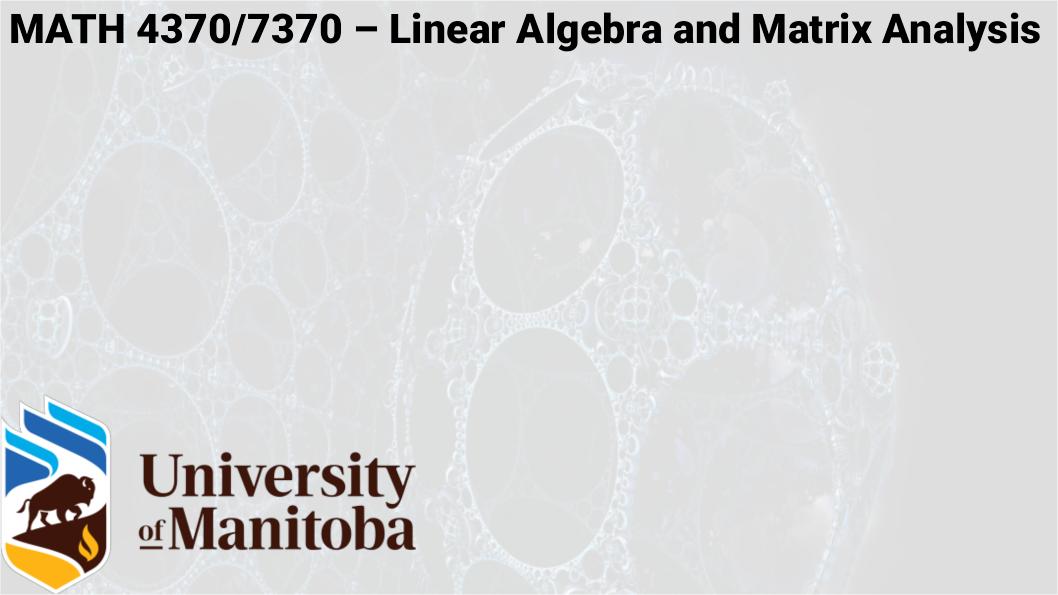
\includegraphics[width=\paperwidth]{title-page-picture.png}
        };
    \end{tikzpicture}
    \titlepage
\end{frame}
\addtocounter{page}{-1}

  
% \begin{frame}
% 	  \tableofcontents[hideallsubsections]
% \end{frame}
% \addtocounter{page}{-1}
  

%%%%%%%%%%%%%%%%%%%%%
%%%%%%%%%%%%%%%%%%%%%
%%%%%%%%%%%%%%%%%%%%%
%%%%%%%%%%%%%%%%%%%%%
% The overall slides outline
{
\setbeamercolor{background canvas}{bg=orange!50}
\begin{frame}[noframenumbering,plain]{\sc Outline of these slides}
    \tableofcontents[onlyparts]
\end{frame}  
}
% \begin{frame}
%   \tableofcontents
%   \foreach\x in {1,...,\totvalue{part}}{%
%       \vskip-0.4cm
%       \tableofcontents[part=\x]%
%   }%
% \end{frame}


\begin{frame}{Source of the material}
    The material in these slides is mostly derived from \cite{Axler2015}
\end{frame}

%%%%%%%%%%%%%%%%%%%%%
%%%%%%%%%%%%%%%%%%%%%
%%%%%%%%%%%%%%%%%%%%%
%%%%%%%%%%%%%%%%%%%%%
%%%%%%%%%%%%%%%%%%%%%
%%%%%%%%%%%%%%%%%%%%%
%%%%%%%%%%%%%%%%%%%%%
%%%%%%%%%%%%%%%%%%%%%
%%%%%%%%%%%%%%%%%%%%%
%%%%%%%%%%%%%%%%%%%%%
%%%%%%%%%%%%%%%%%%%%%
%%%%%%%%%%%%%%%%%%%%%
%\nupart{Some notation and basic stuff}
\nupart{Some notation and basic stuff}

\section{Sets and elements}

\begin{frame}{Sets and elements}
\begin{definition}[Set]
A \defword{set} $X$ is a collection of \defword{elements}.
\end{definition}
We write $x\in X$ or $x\not\in X$ to indicate that the element $x$ belongs to the set $X$ or does not belong to the set $X$, respectively.
\begin{definition}[Subset]
Let $X$ be a set. The set $S$ is a \defword{subset} of $X$, which is denoted
$S\subset X$ or $S\subseteq X$, if all its elements belong to $X$. $S$ is a \defword{proper
subset} of $X$ if it is a subset of $X$ and not equal to $X$; we then write $S\subsetneq X$.
\end{definition}
Smith reserves $\subset$ for $\subsetneq$. I learned $\subset$ for not specified (proper or not) and $\subsetneq$ for proper. So beware!
\end{frame}


\begin{frame}{Quantifiers}
\begin{itemize}
    \item A shorthand notation for ``for all elements $x$ belonging to $X$'' is $\forall x\in X$. For example, if $X=\IR$, the field of real numbers, then $\forall x\in\IR$ means ``for all real numbers $x$''.
    \item A shorthand notation for ``there exists an element $x$ in the set $X$'' is $\exists x\in X$. 
    \item Sometimes we write $\exists!x\in X$ for ``there exists a \defword{unique} $x$ in $X$''.
    \item $\forall$ and $\exists$ are \defword{quantifiers}.
\end{itemize}
\end{frame}

\begin{frame}{Intersection and union of sets}
Let $X$ and $Y$ be two sets.
\begin{definition}[Intersection]
The intersection of $X$ and $Y$, $X\cap Y$, is the set of elements that belong to $X$ \defword{and} to $Y$
\[
X\cap Y=\{x:x\in X\defword{ and } x\in Y\}
\]
\end{definition}
\begin{definition}[Union]
The union of $X$ and $Y$, $X\cup Y$, is the set of elements that belong to $X$ \defword{or} to $Y$
\[
X\cup Y=\{x:x\in X\defword{ or } x\in Y\}
\]
\end{definition}
Use of the expression ``and/or'' is \emph{strictly} forbidden in this course! ``Or but not and'' (a.k.a. \defword{xor}, exclusive or) is $(X\cup Y)\setminus(X\cap Y)$.
\end{frame}



\section{Logic}

\begin{frame}{A few notions of logic}
In a logical sense, a \defword{proposition} is an assertion (or statement)
whose truth value (true or false) can be asserted. For example, a theorem is a
proposition that has been shown to be true. ``The sky is blue'' is also a
proposition. 

Let $A$ be a proposition. We generally write
\[
A
\]
to mean that $A$ is true, and 
\[
\mathbf{not}\ A
\]
to mean that $A$ is false. We also write $\neg A$.
$\mathbf{not}\ A$ is the \defword{negation} of $A$.
\end{frame}


\begin{frame}{A few notions of logic (cont.)}
Let $A,B$ be propositions. Then
\begin{itemize}
\item $A\Rightarrow B$ (read $A$ implies $B$) means that whenever $A$ is true,
then so is $B$.
\item $A\Leftrightarrow B$, also denoted $A$ if and only if $B$ ($A$
iff $B$ for short), means that $A\Rightarrow B$ \defword{and} $B\Rightarrow A$.
We also say that $A$ and $B$ are equivalent.
\end{itemize}
Let $A$ and $B$ be propositions. Then
\[
(A\Rightarrow B)\Leftrightarrow(\mathbf{not}\ B\Rightarrow\mathbf{not}\ A)
\]
This is useful for proving some results.
\end{frame}



\begin{frame}{Necessary and/or sufficient conditions}
Suppose we want to establish whether a given statement $P$ is true, depending
on the truth value of a statement $H$. Then we say that
\begin{itemize}
\item $H$ is a \defword{necessary condition} if $P\Rightarrow H$. \\
(It is necessary that $H$ be true for $P$ to be true; so whenever
$P$ is true, so is $H$).
\item $H$ is a \defword{sufficient condition} if $H\Rightarrow P$. \\
(It suffices for $H$ to be true for $P$ to also be true).
\item $H$ is a \defword{necessary and sufficient condition} if $H\Leftrightarrow
P$, i.e., $H$ and $P$ are equivalent.
\end{itemize}
\end{frame}


\begin{frame}{Playing with quantifiers}
For the quantifiers $\forall$ (for all) and $\exists$ (there exists),
\[
    \exists \text{ is the negation of } \forall
\]
Therefore, for example, the contrapositive of
\[
\forall x\in X,\exists y\in Y
\]
is
\[
\exists x\in X,\forall y\in Y
\]
This is also regularly used in proofs.
\end{frame}


%%%%%%%%%%%%%%%%%%%%%
%%%%%%%%%%%%%%%%%%%%%
%%%%%%%%%%%%%%%%%%%%%
%%%%%%%%%%%%%%%%%%%%%
%%%%%%%%%%%%%%%%%%%%%
%%%%%%%%%%%%%%%%%%%%%
%%%%%%%%%%%%%%%%%%%%%
%%%%%%%%%%%%%%%%%%%%%
%%%%%%%%%%%%%%%%%%%%%
%%%%%%%%%%%%%%%%%%%%%
%%%%%%%%%%%%%%%%%%%%%
%%%%%%%%%%%%%%%%%%%%%
\nupart{Vector spaces}

\section{Fields}

\begin{frame}{Operations}
\begin{definition}[Operations -- Addition and multiplication]
An \defword{operation} on a set $V$ is a mapping that associates an element of the set $V$ to \emph{every} pair of its elements
\begin{itemize}
\item The result of the \defword{addition} of $a$ and $b$ is the \emph{sum} $a+b$ of $a$ and $b$
\item The result of the \defword{multiplication} of $a$ and $b$ is the \emph{product} $ab$ (or $a\cdot b$) of $a$ and $b$
\end{itemize}
\end{definition}
\end{frame}

\begin{frame}{Field}
\begin{definition}[Field]
A \defword{field} is a set $\IF$ together with two (binary) operations, \emph{addition} and \emph{multiplication}, which are required to satisfy the following \emph{field axioms}, where $a,b,c\in\IF$:
\begin{itemize}
\item \defword{Associativity} of addition and multiplication: $a+(b+c)=(a+b)+c$ and $a(bc)=(ab)c$
\item \defword{Commutativity} of addition and multiplication: $a+b=b+a$ and $ab=ba$
\item \defword{Additive} and \defword{multiplicative identity}: $\exists 0,1\in\IF$, $0\neq 1$, s.t. $a+0=a$ and $a1=a$
\item \defword{Additive inverses}: $\forall a\in\IF$, $\exists -a\in\IF$ s.t. $a+(-a)=0$
\item \defword{Multiplicative inverses}: $\forall a\neq 0\in\IF$, $\exists a^{-1}\in\IF$ s.t. $aa^{-1}=1$
\item \defword{Distributivity} (of multiplication over addition): $a(b+c)=(ab)+(ac)$
\end{itemize}
\end{definition}
\end{frame}


\begin{frame}{Notation}
\begin{itemize}
    \item Both $\IR$ and $\IC$ are fields.
    \item From now on, $\IF$ refers to $\IR$ or $\IC$.
    \item Some results are specific to $\IR$ xor $\IC$, in which case we specify the relevant field.
    \item If we use $\IF$, we mean the result applies to both $\IR$ and $\IC$.
\end{itemize}
\end{frame}




%%%%%%%%%%%%%%%%%%%%%
%%%%%%%%%%%%%%%%%%%%%
%%%%%%%%%%%%%%%%%%%%%
%%%%%%%%%%%%%%%%%%%%%
%%%%%%%%%%%%%%%%%%%%%
%%%%%%%%%%%%%%%%%%%%%
\section{Definition of vector spaces}

\begin{frame}{Addition and Scalar multiplication}
\begin{definition}[Addition and scalar multiplication on a set]
\begin{itemize}
\item An \defword{addition} on a set $V$ is a function that assigns an element $\bu+\bv\in V$ to each pair of elements $\bu,\bv\in V$
\item  A \defword{scalar multiplication} on a set $V$ is a function that assigns an element $\lambda \bv$ to each $\lambda\in\IF$ and each $\bv\in V$
\end{itemize}
\end{definition}
\end{frame}

\begin{frame}{Vector space}
\begin{definition}[Vector space]
A \defword{vector space} (over $\IF$) is a set $V$ along with an addition on $V$ and a scalar multiplication on $V$ such that the following properties (\emph{axioms}) hold
\begin{enumerate}
\item $\forall \bu,\bv\in V$, $\bu+\bv=\bv+\bu$  \hfill[\defword{commutativity}]
\item $\forall \bu,\bv,\bw\in V$ and $\forall a,b\in\IF$, $(\bu+\bv)+\bw=\bu+(\bv+\bw)$ and $(ab)\bv=a(b\bv)$ 
\newline\mbox{}\hfill[\defword{associativity}]
\item $\exists \b0_V\in V$ s.t. $\forall \bv\in V$, $\bv+\b0_V=\bv$
\hfill[\defword{additive identity}]
\item $\forall \bv\in V$, $\exists \bw\in V$ s.t. $\bv+\bw=\b0_V$
\hfill[\defword{additive inverse}]
\item $\forall \bv\in V$, $1\bv=\bv$
\hfill[\defword{multiplicative identity}]
\item $\forall a,b\in\IF$ and $\forall \bu,\bv\in V$, 
$a(\bu+\bv)=a\bu+a\bv$ and $(a+b)\bv=a\bv+b\bv$ \newline\mbox{}
\hfill[\defword{distributivity}]
\end{enumerate}
\end{definition}
\end{frame}

\begin{frame}{Results}
\begin{importanttheorem}[Uniqueness of the additive identity]
A vector space $V$ has a unique additive identity $\b0_V\in V$
\end{importanttheorem}
\begin{importanttheorem}[Existence and uniqueness of additive inverse]
Let $V$ be a vector space. Then each $\bv\in V$ has a unique additive inverse, denoted $-\bv$
\end{importanttheorem}
We also define $\bv-\bw$ as $\bv+(-\bw)$.
\begin{theorem}
    \begin{itemize}
    \item $\forall \bv\in V$, $0_\IF \bv=\b0_V$.
    \item $\forall a\ \in\IF$, $a\b0_V=\b0_V$.
    \item $\forall \bv\in V$, $(-1)\bv=-\bv$.
    \end{itemize}
\end{theorem}
\end{frame}
    
\begin{frame}{Vector space}
\begin{definition}[Vector space]
A \defword{vector space} (over $\IF$) is a set $V$ along with an addition on $V$ and a scalar multiplication on $V$ such that the following properties (\emph{axioms}) hold
\begin{enumerate}
\item $\forall \bu,\bv\in V$, $\bu+\bv=\bv+\bu$  \hfill[\defword{commutativity of $+$}]
\item $\forall \bu,\bv,\bw\in V$, $(\bu+\bv)+\bw=\bu+(\bv+\bw)$ \hfill[\defword{associativity of $+$}]
\item $\exists!\b0_V\in V$ s.t. $\forall \bv\in V$, $\bv+\b0_V=\bv$ \hfill[\defword{additive identity}]
\item $\forall \bv\in V$, $\exists!-\bv\in V$ s.t. $\bv+(-\bv)=\b0_V$ \hfill[\defword{additive inverse}]
\item $\forall a\in\IF$ and $\forall \bu,\bv\in V$, $a(\bu+\bv)=a\bu+a\bv$ \hfill[\defword{distributivity of $\cdot$ over $+$}]
\item $\forall a,b\in\IF$ and $\forall \bu\in V$, $(a+b)\bv=a\bv+b\bv$ \hfill[\defword{distributivity of $+$ over $\cdot$}]
\item $\forall a,b\in\IF$, $(ab)\bv=a(b\bv)$ \hfill[\defword{associativity of $\cdot$}]
\item $\forall \bv\in V$, $1\bv=\bv$ \hfill[\defword{multiplicative identity}]
\end{enumerate}
\end{definition}
\end{frame}
            



%%%%%%%%%%%%%%%%%%%%%
%%%%%%%%%%%%%%%%%%%%%
%%%%%%%%%%%%%%%%%%%%%
%%%%%%%%%%%%%%%%%%%%%
%%%%%%%%%%%%%%%%%%%%%
%%%%%%%%%%%%%%%%%%%%%
\section{Example -- Space $\IF^n$}

\begin{frame}{$\IF^n$ is a vector space}
Typically called \emph{Euclidean space} when $\IF=\IR$.
\end{frame}

\begin{frame}
\begin{definition}
Let $0\neq n\in\IN$. An $n$-\defword{tuple} is an ordered collection of $n$ elements,
\[
(x_1,\ldots,x_n)
\]
\end{definition}
\begin{definition}
Let $0\neq n\in\IN$. $\IF^n$ is the set of all $n$-tuples of elements of $\IF$:
\[
\IF^n=\left\{
(x_1,\ldots,x_n): x_j\in\IF\textrm{ for }j=1,\ldots,n
\right\}
\]
\end{definition}
\begin{itemize}
    \item Often write $x=(x_1,\ldots,x_n)$ for short.
    \item For a given $j\in\{1,\ldots,n\}$, $x_j$ is the $j$th \defword{coordinate} of $x$.
    \item Think of $\IR^2,\IR^3,\IR^n$ that you saw in whatever flavour of Linear Algebra 1 you took.
\end{itemize}
\end{frame}


\begin{frame}{Addition in $\IF^n$}
\begin{definition}[Addition in $\IF^n$]
Let $x=(x_1,\ldots,x_n),y=(y_1,\ldots,y_n)\in\IF^n$. Then
\[
x+y=(x_1,\ldots,x_n)+(y_1,\ldots,y_n)=(x_1+y_1,\ldots,x_n+y_n)
\]
\end{definition}
\vfill
\begin{property}[Commutativity of addition in $\IF^n$]
Let $x,y\in\IF^n$, then
\[
x+y=y+x
\]
\end{property}
\end{frame}


\begin{frame}{$0$ and additive inverse in $\IF^n$}
\begin{definition}[$0$]
$0$ denotes the $n$-tuple whose coordinates are all 0,
\[
0=(0,\ldots,0)
\]
\end{definition}
If any ambiguity arises, will write $0_{\IF^n}$
\vfill
\begin{definition}[Additive inverse]
Let $x\in\IF^n$. The \defword{additive inverse} of $x$ is $-x\in\IF^n$ s.t.
\[
x+(-x)=0
\]
\end{definition}
If $x=(x_1,\ldots,x_n)$, then $-x=(-x_1,\ldots,-x_n)$
\end{frame}

\begin{frame}{Scalar multiplication in $\IF^n$}
\begin{definition}[Scalar multiplication]
The \defword{product} of $\lambda\in\IF$ and $x\in\IF^n$ is
\[
\lambda x=\lambda(x_1,\ldots,x_n)=(\lambda x_1,\ldots,\lambda x_n)
\]
\end{definition}
\end{frame}

%%%%%%%%%%%%%%%%%%%%%
%%%%%%%%%%%%%%%%%%%%%
%%%%%%%%%%%%%%%%%%%%%
%%%%%%%%%%%%%%%%%%%%%
%%%%%%%%%%%%%%%%%%%%%
%%%%%%%%%%%%%%%%%%%%%
\section{Example -- Complex numbers}

\begin{frame}{Complex numbers}
\begin{definition}[Complex numbers]
A \defword{complex number} is an ordered pair $(a,b)$, where $a,b\in\IR$. Usually written $a+ib$ or $a+bi$, where $i^2=-1$

The set of all complex numbers is denoted $\IC$, 
\[
\IC=\{a+ib: a,b\in\IR\}
\]
\end{definition}
\end{frame}

\begin{frame}
\begin{definition}[Addition and multiplication on $\IC$]
Letting $a+ib$ and $c+id\in\IC$, addition on $\IC$ is defined by
\[
(a+ib)+(c+id) = (a+c)+i(b+d)
\]
and multiplication on $\IC$ is defined by
\[
(a+ib)(c+id) = (ac-bd)+i(ad+bc)
\]
\end{definition}
Latter equality easy to obtain using regular multiplication and $i^2=-1$
\end{frame}

\begin{frame}{Properties}
$\forall\alpha,\beta,\gamma\in\IC$,
\begin{itemize}
\item $\alpha+\beta=\beta+\alpha$ and $\alpha\beta=\beta\alpha$ \hfill[\defword{commutativity}]
\item $(\alpha+\beta)+\gamma=\alpha+(\beta+\gamma)$ and $(\alpha\beta)\gamma=\alpha(\beta\gamma)$ \hfill[\defword{associativity}]
\item $\gamma+0=\gamma$ and $\gamma 1=\gamma$ \hfill[\defword{identities}]
\item $\forall\alpha\in\IC$, $\exists\beta\in\IC$ unique s.t. $\alpha+\beta=0$ \hfill[\defword{additive inverse}]
\item $\forall \alpha\neq 0\in\IC$, $\exists\beta\in\IC$ unique s.t. $\alpha\beta=1$ \hfill[\defword{multiplicative inverse}]
\item $\gamma(\alpha+\beta)=\gamma\alpha+\gamma\beta$ \hfill[\defword{distributivity}]
\end{itemize}
Thus $\IC$ is a field.
\end{frame}


\begin{frame}{Additive \& multiplicative inverse, subtraction, division}
\begin{definition}
Let $\alpha,\beta\in\IC$
\begin{itemize}
\item $-\alpha$ is the \defword{additive inverse} of $\alpha$, i.e., the unique number in $\IC$ s.t. $\alpha+(-\alpha)=0$
\item \defword{Subtraction} on $\IC$:
\[
\beta-\alpha=\beta+(-\alpha)
\]
\item For $\alpha\neq 0$, $1/\alpha$ is the \defword{multiplicative inverse} of $\alpha$, i.e., the unique number in $\IC$ s.t.
\[
\alpha(1/\alpha)=1
\]
\item \defword{Division} on $\IC$:
\[
\beta/\alpha=\beta(1/\alpha)
\]
\end{itemize}
\end{definition}
\end{frame}


\begin{frame}
\begin{definition}[Real and imaginary parts]
Let $z=a+ib$. Then $\Re z=a$ is \defword{real part} and $\Im z=b$ is \defword{imaginary part} of $z$
\end{definition}
If ambiguous, write $\Re(z)$ and $\Im(z)$
\begin{definition}[Conjugate and Modulus]
Let $z=a+ib\in\IC$. Then
\begin{itemize}
\item \defword{Complex conjugate} of $z$ is
\[
\bar z=\Re z-i(\Im z) = a-ib
\]
\item \defword{Modulus} (or \defword{absolute value}) of $z$ is
\[
|z|=\sqrt{\left(\Re z\right)^2+\left(\Im z\right)^2} = \sqrt{a^2+b^2} \geq 0
\]
\end{itemize}
\end{definition}
\end{frame}

\begin{frame}{Properties of complex numbers}
Let $w,z\in\IC$, then
\begin{itemize}
\item $z+\bar z=2\Re z$
\item $z-\bar z=2i\Im z$
\item $z\bar z=|z|^2$
\item $\overline{w+z}=\bar w+\bar z$ and $\overline{wz}=\bar w\bar z$
\item $\overline{\bar z}=z$
\item $|\Re z|\leq |z|$ and $|\Im z|\leq |z|$
\item $|\bar z|=|z|$
\item $|wz|=|w|\;|z|$
\item $|w+z|\leq |w|+|z|$ \hfill[\defword{triangle inequality}]
\end{itemize}
\end{frame}



%%%%%%%%%%%%%%%%%%%%%
%%%%%%%%%%%%%%%%%%%%%
%%%%%%%%%%%%%%%%%%%%%
%%%%%%%%%%%%%%%%%%%%%
%%%%%%%%%%%%%%%%%%%%%
%%%%%%%%%%%%%%%%%%%%%
\section{Subspaces}

\begin{frame}{Subspace}
\begin{definition}[Subspace]
\label{def:subspace}
Let $V$ be a vector space over $\IF$. Let $U\subseteq V$ be a subset of $V$. Then $U$ is a \defword{subspace} of $V$ if $U$ is a vector space over $\IF$ for the same operations of addition and scalar multiplication as $V$
\end{definition}
\begin{importanttheorem}[Conditions for a subspace]
\label{th:conditions_subspace}
$U\subseteq V$ is a subspace of $V$ $\iff$ $U$ satisfies the following three conditions:
\begin{itemize}
    \item $\b0_V\in U$ \hfill[\defword{additive identity}]
    \item $\forall \bu,\bv\in U$, $\bu+\bv\in U$ 
    \hfill[\defword{closed under addition}]
    \item $\forall \bu\in U$, $\forall a\in\IF$, $a\bu\in U$
    \hfill[\defword{closed under scalar multiplication}]
\end{itemize}
\end{importanttheorem}
The smallest possible subspace of $V$ is $\{\b0_V\}$, the largest is $V$.
\end{frame}



\begin{frame}{Sums of subspaces}
\begin{definition}[Sum of subsets]
Let $V$ be a vector space and $U_1,\ldots,U_m$ be \emph{subsets} of $V$. The \defword{sum} of $U_1,\ldots,U_m$ is
\[
U_1+\cdots+U_m=
\left\{
\bu_1+\cdots+\bu_m: \bu_1\in U_1,\ldots,\bu_m\in U_m
\right\}
\]
\end{definition}
\vfill
\begin{theorem}
Let $V$ be a vector space and $U_1,\ldots,U_m$ be \emph{subspaces} of $V$. Then $U_1+\cdots+U_m$ is the smallest subspace of $V$ containing $U_1,\ldots,U_m$
\end{theorem}
\end{frame}

\begin{frame}{Direct sums}
\begin{definition}[Direct sum]
Suppose $U_1,\ldots,U_m$ are subspaces of a vector space $V$.
The sum $U_1+\cdots+U_m$ is a \defword{direct sum} and is then written $U_1\oplus\cdots\oplus U_m$ if each element of $U_1+\cdots+U_m$ can be written in only one way as a sum $\bu_1+\cdots+\bu_m$, where each $\bu_j\in U_j$
\end{definition}
\vfill
\begin{theorem}[Condition for a direct sum]
Suppose $U_1,\ldots,U_m$ are subspaces of a vector space $V$. 
Then $U_1+\cdots+U_m$ is a direct sum $\iff$ the only way to write $\b0$ as a sum $\bu_1+\cdots+\bu_m$, where each $\bu_j\in U_j$, is by taking each $\bu_j$ equal to $\b0_V$
\end{theorem}
\vfill
\begin{importanttheorem}[Direct sum of two subspaces]
Let $U,W$ be subspaces of a vector space $V$. Then $U+W$ is a direct sum $\iff$ $U\cap W=\{\b0_V\}$
\end{importanttheorem}
\end{frame}


%%%%%%%%%%%%%%%%%%%%%
%%%%%%%%%%%%%%%%%%%%%
%%%%%%%%%%%%%%%%%%%%%
%%%%%%%%%%%%%%%%%%%%%
%%%%%%%%%%%%%%%%%%%%%
%%%%%%%%%%%%%%%%%%%%%
%%%%%%%%%%%%%%%%%%%%%
%%%%%%%%%%%%%%%%%%%%%
%%%%%%%%%%%%%%%%%%%%%
%%%%%%%%%%%%%%%%%%%%%
%%%%%%%%%%%%%%%%%%%%%
%%%%%%%%%%%%%%%%%%%%%
\nupart{Finite-dimensional vector spaces}

%%%%%%%%%%%%%%%%%%%%%
%%%%%%%%%%%%%%%%%%%%%
%%%%%%%%%%%%%%%%%%%%%
%%%%%%%%%%%%%%%%%%%%%
%%%%%%%%%%%%%%%%%%%%%
%%%%%%%%%%%%%%%%%%%%%
\section{Span and Linear independence}

\begin{frame}
\begin{definition}[Linear combination]
A \defword{linear combination} of a list $\bv_1,\ldots,\bv_m$ of vectors in $V$ is a vector
\[
a_1\bv_1+\cdots+a_m\bv_m,
\]
where $a_1,\ldots,a_m\in\IF$
\end{definition}
\begin{definition}[Span]
The set of all linear combinations of a list of vectors $\bv_1,\ldots,\bv_m$ is the \defword{span} of $\bv_1,\ldots,\bv_m$,
\[
\Span(\bv_1,\ldots,\bv_m)=
\left\{
a_1\bv_1+\cdots+a_m\bv_m:a_1,\ldots,a_m\in\IF
\right\}
\]
The span of the empty list $(\;)$ is $\{\b0_V\}$
\end{definition}
\end{frame}


\begin{frame}{Finite/infinite-dimensional vector spaces}
\begin{theorem}
The span of a list of vectors in $V$ is the smallest subspace of $V$ containing all the vectors in the list
\end{theorem}
\begin{definition}[List of vectors spanning a space]
If $\Span(\bv_1,\ldots,\bv_m)=V$, we say $\bv_1,\ldots,\bv_m$ \defword{spans} $V$
\end{definition}
\begin{definition}[Finite-dimensional vector space]
A vector space $V$ is \defword{finite-dimensional} if some list of vectors in it spans $V$
\end{definition}
\begin{definition}[Infinite-dimensional vector space]
A vector space $V$ is \defword{infinite-dimensional} if it is not finite-dimensional
\end{definition}
\end{frame}


\begin{frame}{Linear (in)dependence}
\begin{definition}[Linear independence/Linear dependence]
A list $\bv_1,\ldots,\bv_m$ of vectors in a vector space $V$ is \defword{linearly independent} if
\[
\left(a_1\bv_1+\cdots+a_m\bv_m=0\right)
\Leftrightarrow
\left(a_1=\cdots=a_m=0\right),
\]
where $a_1,\ldots,a_m\in\IF$. 
A list of vectors is \defword{linearly dependent} if it is not linearly independent.
\end{definition}
The empty list $(\;)$ is assumed to be linearly independent
\end{frame}


\begin{frame}
\begin{lemma}[Linear dependence]
Let $\bv_1,\ldots,\bv_m$ be a \emph{linearly dependent} list in a vector space $V$. Then there exists $j\in\{1,2,\ldots,m\}$ s.t.
\begin{enumerate}
\item $\bv_j\in\Span(\bv_1,\ldots,\bv_{j-1})$
\item if the $j$th term is removed from $\bv_1,\ldots,\bv_m$, the span of the remaining list equals $\Span(\bv_1,\ldots,\bv_m)$
\end{enumerate}
\end{lemma}
\begin{importanttheorem}
Let $V$ be a finite-dimensional vector space. Then the length of every linearly independent list of vectors is less than or equal to the length of every spanning list of vectors
\end{importanttheorem}
\begin{importanttheorem}[Subspace of a finite-dimensional vector space]
Every subspace of a finite-dimensional vector space is finite-dimensional
\end{importanttheorem}
\end{frame}


%%%%%%%%%%%%%%%%%%%%%
%%%%%%%%%%%%%%%%%%%%%
%%%%%%%%%%%%%%%%%%%%%
%%%%%%%%%%%%%%%%%%%%%
%%%%%%%%%%%%%%%%%%%%%
%%%%%%%%%%%%%%%%%%%%%
\section{Bases}

\begin{frame}{Basis}
\begin{definition}[Basis]
Let $V$ be a vector space. A \defword{basis} of $V$ is a list of vectors in $V$ that is both linearly independent and spanning
\end{definition}

\begin{theorem}[Criterion for a basis]
A list $\bv_1,\ldots,\bv_m$ of vectors in a vector space $V$ is a basis of $V$ iff $\forall \bv\in V$, $v$ can be written uniquely in the form
\[
\bv=a_1\bv_1+\cdots+a_m\bv_m,
\]
where $a_1,\ldots,a_m\in\IF$
\end{theorem}
\end{frame}

\begin{frame}
\begin{importanttheorem}[All spanning lists contain a basis]
Every spanning list in a vector space can be reduced to a basis of the vector space
\end{importanttheorem}

\begin{importanttheorem}[Basis of finite-dimensional vector space]
Every finite-dimensional vector space has a basis
\end{importanttheorem}

\begin{importanttheorem}[Extension to a basis]
Every linearly independent list of vectors in a finite-dimensional vector space can be extended to a basis of the vector space
\end{importanttheorem}

\begin{theorem}
Let $V$ be a finite-dimensional vector space and $U\subset V$ be a subspace of $V$. Then $\exists W\subset V$ subspace of $V$ s.t. $V=U\oplus W$
\end{theorem}
\end{frame}


%%%%%%%%%%%%%%%%%%%%%
%%%%%%%%%%%%%%%%%%%%%
%%%%%%%%%%%%%%%%%%%%%
%%%%%%%%%%%%%%%%%%%%%
%%%%%%%%%%%%%%%%%%%%%
%%%%%%%%%%%%%%%%%%%%%
\section{Dimension}

\begin{frame}
\begin{importanttheorem}[Bases of a finite-dim. space have equal length]
Any two bases of a finite-dimensional vector space have the same length
\end{importanttheorem}

\begin{definition}[Dimension]
The \defword{dimension} $\dim V$ of a finite-dimensional vector space $V$ is the length of any basis of the vector space
\end{definition}

\begin{importanttheorem}[Dimension of a subspace]
Let $V$ be a finite-dimensional vector space and $U\subset V$ be a subspace of $V$. Then $\dim U\leq \dim V$
\end{importanttheorem}
\end{frame}


\begin{frame}
\begin{importanttheorem}
Let $V$ be a finite-dimensional vector space. Then every linearly independent list of vectors in $V$ with length $\dim V$ is a basis of $V$
\end{importanttheorem}

\begin{importanttheorem}
Let $V$ be a finite-dimensional vector space. Then every spanning list of vectors in $V$ with length $\dim V$ is a basis of $V$
\end{importanttheorem}

\begin{importanttheorem}[Dimension of a sum of subspaces]
Let $U_1,U_2$ be subspaces of a finite-dimensional vector space $V$. Then
\[
\dim\left(U_1+U_2\right)=\dim U_1+\dim U_2-\dim\left(U_1\cap U_2\right)
\]
\end{importanttheorem}
\end{frame}


%%%%%%%%%%%%%%%%%%%%%
%%%%%%%%%%%%%%%%%%%%%
%%%%%%%%%%%%%%%%%%%%%
%%%%%%%%%%%%%%%%%%%%%
%%%%%%%%%%%%%%%%%%%%%
%%%%%%%%%%%%%%%%%%%%%
%%%%%%%%%%%%%%%%%%%%%
%%%%%%%%%%%%%%%%%%%%%
%%%%%%%%%%%%%%%%%%%%%
%%%%%%%%%%%%%%%%%%%%%
%%%%%%%%%%%%%%%%%%%%%
%%%%%%%%%%%%%%%%%%%%%
\nupart{Linear maps}


%%%%%%%%%%%%%%%%%%%%%
%%%%%%%%%%%%%%%%%%%%%
%%%%%%%%%%%%%%%%%%%%%
%%%%%%%%%%%%%%%%%%%%%
%%%%%%%%%%%%%%%%%%%%%
%%%%%%%%%%%%%%%%%%%%%
\section{Vector space of linear maps}


\begin{frame}
\begin{definition}[Linear map/transformation]
Let $V,W$ be vector spaces. A \defword{linear map} (or \defword{linear transformation}) from $V$ to $W$ is a function $T:V\to W$ that has the following properties:
\begin{enumerate}
\item \defword{Additivity} $\forall \bu,\bv\in V$, $T(\bu+\bv)=T(\bu)+T(\bv)$.
\item \defword{Homogeneity} $\forall\lambda\in\IF$, $\forall \bv\in V$, $T(\lambda \bv)=\lambda T(\bv)$.
\end{enumerate}
\end{definition}
\vfill
Often, parentheses are omitted, $T(\bu)$ is written $T\bu$
\vfill
The set of all linear maps from $V$ to $W$ is denoted $\L(V,W)$
\end{frame}


\begin{frame}
\begin{importanttheorem}[Linear maps and basis of domain]
Let $V,W$ be two vector spaces and $\bv_1,\ldots,\bv_n$ be a basis of $V$. Let $\bw_1,\ldots,\bw_n\in W$. Then there exists a unique linear map $T:V\to W$ s.t.
\[
\forall j=1,\ldots,n,\qquad T\bv_j=\bw_j
\]
\end{importanttheorem}
\end{frame}


\begin{frame}
\begin{definition}[Addition \& Scalar multiplication]
\label{def:add_scalar_mult_linear_maps}
Let $V,W$ be vector spaces, $S,T\in\L(V,W)$ and $\lambda\in\IF$. 
The \defword{sum} $S+T$ and \defword{product} $\lambda T$ are the linear maps from $V$ to $W$ defined, $\forall \bv\in V$, by
\[
(S+T)(\bv)=S\bv+T\bv\textrm{ and }(\lambda T)(\bv)=\lambda(T\bv).
\]
\end{definition}
\vfill
\begin{importanttheorem}[Linear maps are vector spaces]
Let $V,W$ be vector spaces. Equipped with addition and scalar multiplication as just defined, $\L(V,W)$ is a vector space.
\end{importanttheorem}
\end{frame}

\begin{frame}{Product of linear maps}
\begin{definition}[Product of linear maps]
Let $U,V,W$ be vector spaces, $T\in\L(U,V),S\in\L(V,W)$. The \defword{product} $ST\in\L(U,W)$ is defined for $\bu\in U$ by
\[
(ST)(\bu)=S(T\bu).
\]
\end{definition}
This means that the product of linear maps is the composition $S\circ T$, although because of the linearity, we often omit the $\circ$ composition sign.
\end{frame}

\begin{frame}{Properties of products of linear maps}
\begin{theorem}
\begin{enumerate}
\item \defword{Associativity} If $V,V_2,V_3,W$ vector spaces, $T_1\in\L(V,V_2),T_2\in\L(V_2,V_3),T_3\in\L(V_3,W)$, then
\[
(T_1T_2)T_3=T_1(T_2T3)
\]
\item \defword{Identity} $V,W$ vector spaces. Then for $T\in\L(V,W)$,
\[
TI_V=I_WT=T
\]
\item \defword{Distributivity} $U,V,W$ vector spaces, $T,T_1,T_2\in\L(U,V),S,S_1,S_2\in\L(V,W)$, then
\[
(S_1+S_2)T=S_1T+S_2T\textrm{ and }S(T_1+T_2)=ST_1+ST_2
\]
\end{enumerate}
\end{theorem}
\end{frame}


\begin{frame}
\begin{theorem}[Linear maps take 0 to 0]
Let $V,W$ be vector spaces, $T\in\L(V,W)$. Then
\[
T(\b0_V)=\b0_W.
\]
\end{theorem}
\end{frame}


%%%%%%%%%%%%%%%%%%%%%
%%%%%%%%%%%%%%%%%%%%%
%%%%%%%%%%%%%%%%%%%%%
%%%%%%%%%%%%%%%%%%%%%
%%%%%%%%%%%%%%%%%%%%%
%%%%%%%%%%%%%%%%%%%%%
\section{Null spaces and Ranges}


\begin{frame}
\begin{definition}[Null space]
Let $V,W$ be finite-dimensional vector spaces and $T\in\L(V,W)$. The \defword{null space} $\nullspace T$ (or \defword{kernel} $\ker T$) of $T$ is the subet of $V$ consisting of those vectors that $T$ maps to $\b0_W$:
\[
\nullspace T=\left\{\bv\in V; T\bv=\b0_W \right\}.
\]
\end{definition}
\begin{importanttheorem}[Null space is a subspace]
Let $V,W$ be finite-dimensional vector spaces and $T\in\L(V,W)$.
Then $\nullspace T$ is a subspace of $V$
\end{importanttheorem}
\end{frame}


\begin{frame}
\begin{definition}[Injectivity]
A function $T:V\to W$ is \defword{injective} (or \defword{one-to-one}) if
\[
T\bu=T\bv \Rightarrow \bu=\bv.
\]
\end{definition}
We can also use the contrapositive: $T$ injective if $\bu\neq \bv\Rightarrow T\bu\neq T\bv$.
\begin{importanttheorem}[Linking injectivity and null space]
Let $V,W$ be finite-dimensional vector spaces, $T\in\L(V,W)$. Then 
\[
T\textrm{ injective}\Leftrightarrow \nullspace T=\{\b0_V\}
\]
\end{importanttheorem}
\end{frame}


\begin{frame}
\begin{definition}[Range]
Let $V,W$ be finite-dimensional vector spaces, $T:V\to W$ a function. The \defword{range} (or \defword{image}) of $T$ is the subset of $W$ defined by
\[
\range\ T=\{T\bv;\bv\in V\}.
\]
\end{definition}
When talking about the image, we write $\mathsf{Im}\ T$.
\vfill
\begin{importanttheorem}[Range is a subspace]
Let $V,W$ be finite-dimensional vector spaces, $T\in\L(V,W)$. Then $\range T$ is a subspace of $W$.
\end{importanttheorem}

\end{frame}

\begin{frame}
\begin{definition}[Surjectivity]
A function $T:V\to W$ is \defword{surjective} (or \defword{onto}) if
\[
\range T=W
\]
\end{definition}
\vfill
\begin{importanttheorem}[Fundamental theorem of linear maps]
Let $V$ be a finite-dimensional vector space and $T\in\L(V,W)$. Then $\dim\range T<\infty$ and
\[
\dim V=\dim\nullspace T+\dim\range T
\]
\end{importanttheorem}
\end{frame}


\begin{frame}
\begin{importanttheorem}[Linear map onto a smaller space is not injective]
Let $V,W$ be finite-dimensional vector spaces such that $\dim V>\dim W$. Then $\nexists T\in\L(V,W)$ that is injective
\end{importanttheorem}
\vfill
\begin{importanttheorem}[Linear map onto a larger space is not surjective]
Let $V,W$ be finite-dimensional vector spaces such that $\dim V<\dim W$. Then $\nexists T\in\L(V,W)$ that is surjective
\end{importanttheorem}
\end{frame}



\begin{frame}{Do as exercises..}
\begin{theorem}
A homogeneous system of linear equations with more variables than equations has nonzero solutions.
\end{theorem}
\vfill
\begin{theorem}
A nonhomogeneous system of linear equations with more equations than variables has no solution for some choice of the constant terms
\end{theorem}
\end{frame}



%%%%%%%%%%%%%%%%%%%%%
%%%%%%%%%%%%%%%%%%%%%
%%%%%%%%%%%%%%%%%%%%%
%%%%%%%%%%%%%%%%%%%%%
%%%%%%%%%%%%%%%%%%%%%
%%%%%%%%%%%%%%%%%%%%%
\section{Matrices}


\begin{frame}
\begin{definition}[Matrix]
An $m$-by-$n$ or $m\times n$ matrix is a rectangular array of elements of $\IF$ with $m$ rows and $n$ columns,
\[
A=[a_{ij}]=
\begin{pmatrix}
a_{11} & \cdots & a_{1n} \\
\vdots & & \vdots \\
a_{m1} & \cdots & a_{mn}
\end{pmatrix}
\]
\end{definition}

Remember that we always list indices as ``row,column''

We denote $\M_{mn}(\IF)$ the set of $m\times n$ matrices with entries in $\IF$
\end{frame}


\begin{frame}
\begin{definition}[Matrix of a linear map]
Let $V,W$ be finite-dimensional vector spaces, $v_1,\ldots,v_n$ a basis of $V$ and $w_1,\ldots,w_m$ a basis of $W$. The \defword{matrix of} $T$ with respect to these bases is the matrix $M(T)\in\M_{mn}$ with entries $a_{jk}$ defined by
\[
Tv_k = a_{1k}w_1+\cdots +a_{mk}w_m
\]
for $1\leq l\leq n$.
If the bases are not clear from the context, then write
\[
M(T,(v_1,\ldots,v_n),(w_1,\ldots,w_m))
\]
\end{definition}
I will often write $M_T$ rather than $M(T)$.
\end{frame}


\begin{frame}
Most definitions are assumed known

\begin{theorem}[Matrix of sums of linear maps]
Suppose $S,T\in\L(V,W)$. Then $M(S+T)=M(S)+M(T)$
\end{theorem}

\begin{theorem}[Matrix of a scalar times a linear map]
Suppose $T\in\L(V,W)$, $\lambda\in\IF$. Then $M(\lambda T)=\lambda M(T)$
\end{theorem}

\begin{theorem}[Dimension of $\M_{mn}$]
$\dim \IF^{mn}=mn$
\end{theorem}

\begin{theorem}[Matrix of products of linear maps]
Suppose $T\in\L(U,V),S\in\L(V,W)$. Then $M(ST)=M(S)M(T)$
\end{theorem}
\end{frame}


\begin{frame}
\begin{theorem}
Let $A\in\M_{mn}$, $C\in\M_{np}$. Then
\[
(AC)_{jk}=A_{j\bullet}C_{\bullet k},\qquad 1\leq j\leq m,1\leq k\leq p
\]
and
\[
(AC)_{\bullet k}=AC_{\bullet k},\qquad 1\leq k\leq p
\]
\end{theorem}
\vfill
\begin{theorem}
Let $A\in\M_{mn}$, $c=(c_1,\ldots,c_n)^T\in\M_{n1}$. Then
\[
Ac = c_1A_{\bullet 1}+\cdots+c_nA_{\bullet n}
\]
\end{theorem}
\end{frame}

\begin{frame}{Change of basis}
\begin{definition}[Change of basis matrix]
$\B=\{\bu_1,\ldots,\bu_n\}$ and $\C=\{\bv_1,\ldots,\bv_n\}$ bases of vector space $V$
The \defword{change of basis matrix} $P_{\C\leftarrow\B}\in\M_n$,
\[
P_{\C\leftarrow\B}
=\left[
[\bu_1]_\C \cdots [\bu_n]_\C
\right]
\]
has columns the coordinate vectors $[\bu_1]_\C,\ldots,[\bu_n]_\C$ of the vectors in $\B$ w.r.t. $\C$
\end{definition}
\vfill
\begin{theorem}
$\B=\{\bu_1,\ldots,\bu_n\}$ and $\C=\{\bv_1,\ldots,\bv_n\}$ bases of vector space $V$ and $P_{\C\leftarrow\B}$ a change of basis matrix from $\B$ to $\C$
\begin{enumerate}
\item $\forall\bx\in V$, $P_{\C\leftarrow\B}[\bx]_\B = [\bx]_\C$
\item $P_{\C\leftarrow\B}$ s.t. $\forall\bx\in V$, $P_{\C\leftarrow\B}[\bx]_\B = [\bx]_\C$ is \defword{unique}
\item $P_{\C\leftarrow\B}$ invertible and $P_{\C\leftarrow\B}^{-1}=P_{\B\leftarrow\C}$
\end{enumerate}
\end{theorem}
\end{frame}

\begin{frame}{Row-reduction method for changing bases}
\begin{theorem}
$\B=\{\bu_1,\ldots,\bu_n\}$ and $\C=\{\bv_1,\ldots,\bv_n\}$ bases of vector space $V$. Let $\E$ be any basis for $V$,
\[
B = [[\bu_1]_\E,\ldots,[\bu_n]_\E] 
\textrm{ and }
C = [[\bv_1]_\E,\ldots,[\bv_n]_\E] 
\]
and let $[C|B]$ be the augmented matrix constructed using $C$ and $B$. Then
\[
RREF\left([C|B]\right)
=[\II|P_{\C\leftarrow\B}]
\]
\end{theorem}

If working in $\IR^n$, this is quite useful with $\E$ the standard basis of $\IR^n$ (it does not matter if $\B=\E$)
\end{frame}


\begin{frame}{More on changing bases}
    \begin{theorem}[NSC for two matrices representing the same linear map]
        Let $A,B\in\M_{mn}$, $V$ and $W$ be $n$ and $m$ dimensional vector spaces, respectively. Then $A$ and $B$ represent the same linear transformation $T\in\L(V,W)$ relative to perhaps different bases of $V$ and $W$ $\iff$ $\exists P\in\M_m$, $Q\in\M_n$ nonsingular and such that
        \[
        A=PBQ^{-1}
        \]
    \end{theorem}
\end{frame}


%%%%%%%%%%%%%%%%%%%%%
%%%%%%%%%%%%%%%%%%%%%
%%%%%%%%%%%%%%%%%%%%%
%%%%%%%%%%%%%%%%%%%%%
%%%%%%%%%%%%%%%%%%%%%
%%%%%%%%%%%%%%%%%%%%%
\section{Invertibility and Isomorphic vector spaces}


\begin{frame}
\begin{definition}[Inverse/Invertibility]
$T\in\L(V,W)$ is \defword{invertible} if $\exists S\in\L(W,V)$ s.t. $ST=I_V$ and $TS=I_W$. Such a map is the \defword{inverse} of $T$
\end{definition}

\begin{importanttheorem}[Uniqueness of inverse]
An invertible linear map $T\in\L(V,W)$ has a unique inverse denoted $T^{-1}$
\end{importanttheorem}

\begin{importanttheorem}[NSC for invertibility]
$T\in\L(V,W)$ invertible $\Leftrightarrow$ ($T$ injective and surjective)
\end{importanttheorem}
\end{frame}


\begin{frame}
\begin{definition}[Isomorphism/Isomorphic spaces]
$T\in\L(V,W)$ is an \defword{isomorphism} if it invertible. Two vector spaces are \defword{isomorphic} if there exists an isomorphism from one to the other
\end{definition}

\begin{importanttheorem}[NSC for isomorphicity]
Let $V,W$ be finite-dimensional vector spaces over $\IF$. Then 
\[
V \textrm{ and } W \textrm{ are isomorphic}
\Leftrightarrow \dim V=\dim W
\]
\end{importanttheorem}

\begin{theorem}
Let $v_1,\ldots,v_n$ be a basis of $V$ and $w_1,\ldots,w_m$ be a basis of $W$. Then $M$ is an isomorphism between $\M_{mn}$ and $\L(V,W)$
\end{theorem}
\end{frame}


\begin{frame}
\begin{importanttheorem}[Dimension of $\L(V,W)$]
Let $V,W$ be finite-dimensional vector spaces. Then $\L(V,W)$ is finite-dimensional and 
\[
\dim \L(V,W)=\dim V\; \dim W
\]
\end{importanttheorem}
\end{frame}

\begin{frame}
\begin{definition}[Matrix of a vector]
Let $V$ be a finite-dimensional vector space, $v\in V$ and $v_1,\ldots,v_n$ a basis of $V$. The \defword{matrix} of $v$ with respect to the basis $v_1,\ldots,v_n$ is the $n\times 1$ matrix
\[
M(v)=\begin{pmatrix}
c_1\\
\vdots\\
c_n
\end{pmatrix}
\]
where $c_1,\ldots,c_n\in\IF$ are s.t.
\[
v=c_1v_1+\cdots+c_nv_n
\]
\end{definition}
\begin{theorem}
Let $V,W$ be finite-dimensional vector spaces, $v_1,\ldots,v_n$ a basis of $V$, $w_1,\ldots,w_m$ a basis of $W$ and $T\in\L(V,W)$. For $k\in\{1,\ldots,n\}$, $M(T)_{\bullet k}=M(Tv_k)$
\end{theorem}
\end{frame}

\begin{frame}
\begin{theorem}[Linear maps act like matrix multiplication]
Let $V,W$ be finite-dimensional vector spaces, $v_1,\ldots,v_n$ a basis of $V$, $w_1,\ldots,w_m$ a basis of $W$, $T\in\L(V,W)$ and $v\in V$. Then
\[
M(Tv)=M(T)M(v)
\]
\end{theorem}
\end{frame}

\begin{frame}{Operator/Endomorphism}
\begin{definition}[Operator/Endomorphism]
    Let $V$ be a vector space. A linear map $\L(V,V)$ is an \defword{operator} (or an \defword{endomorphism}). $\L(V)=\L(V,V)$ denotes the set of all operators on $V$
\end{definition}
\vfill
\begin{importanttheorem}[Injectivity equiv. to surjectivity in finite-dim.]
Let $V$ be a finite-dimensional vector space, $T\in\L(V)$. TFAE:
\begin{enumerate}
\item $T$ invertible
\item $T$ injective
\item $T$ surjective
\end{enumerate}
\end{importanttheorem}
\end{frame}


\begin{frame}{Rank of an operator/endomorphism}
    \begin{proposition}[Rank]
        Let $T\in\L(V)$ with $V$ finite-dimensional. Then there exists bases $\B_U=\{u_1,\ldots,u_n\}$ and $\B_V=\{v_1,\ldots,v_n\}$ for $V$ such that the matrix $M_T$ of $T$ can be written as the block matrix
        \[
        M_T=\begin{pmatrix}
            \diag(1,\ldots,1) & \b0_{k,n-k} \\
            \b0_{n-k,k} & \b0_{n-k,n-k}
        \end{pmatrix}
\]
        for some $k\in\IN$ called the \defword{rank} of $T$, with $k=\rank(T)=\dim(\range\ T)$.
    \end{proposition}
\end{frame}

\begin{frame}
    \begin{definition}[Row and column rank]
        Let $A\in\M_{mn}(\IF)$ be a matrix
        \begin{itemize}
            \item The \defword{row rank} of $A$ is the dimension of the span of the rows of $A$ in $\M_{1n}(\IF)$
            \item The \defword{column rank} of $A$ is the dimension of the span of the columns of $A$ in $\M_{m1}(\IF)$
        \end{itemize}
    \end{definition}
    Row and column ranks are the dimensions of the row and column spaces of Definition~\ref{def:row_column_spaces}.
\end{frame}

\begin{frame}
    \begin{theorem}[$\dim\range T$ equals column rank of $M(T)$]
        Let $V,W$ be finite-dimensional vector spaces, $T\in\L(V,W)$. Then $\dim\range T$ equals the column rank of $M(T)$
    \end{theorem}
    \vfill
    \begin{theorem}[Row rank equals column rank]\label{th:row_rank_equals_column_rank}
        Let $A\in\M_{mn}$. Then the row rank of $A$ equals the column rank of $A$
    \end{theorem}
    \vfill
    \begin{definition}[Rank]
        Let $A\in\M_{mn}(\IF)$. The \defword{rank} of $A$ is the column (or row, by Theorem~\ref{th:row_rank_equals_column_rank}) rank of $A$
    \end{definition}
\end{frame}

\begin{frame}{Row space and column space of a matrix}
    \begin{definition}[Row and column spaces]\label{def:row_column_spaces}
        Let $A\in\M_{mn}$. The subspaces of $\IR^n$ and $\IR^m$ spanned by the row and column vectors of $A$ are the \defword{row space} and \defword{column space} of $A$, respectively.
    \end{definition}
    \begin{definition}[Null space/kernel]
        Let $A\in\M_{mn}$. The null space (or kernel) of $A$ is the solution space of the homogeneous system $A\bx=\b0$.
    \end{definition}
    This makes explicit the already seen definition in the special case of a matrix. As previously seen, the null space is a subspace of $\IR^n$.
    \begin{definition}[Nullity]
        The dimension of the null space of $A\in\M_{mn}$ is called the \defword{nullity} of $A$.
    \end{definition}
\end{frame}

\begin{frame}
    \begin{theorem}
        Let $A\in\M_{mn}$. Then
        \begin{enumerate}
            \item $\rank(A)=\rank(A^T)$
            \item $\rank(A)+\nullity(A)=n$
            \item $\rank(A)\leq\min(m,n)$
        \end{enumerate}
    \end{theorem}
    \vfill
    \begin{theorem}[Consistency]
        Consider the linear system $A\bx=\bb$, with $A\in\M_{mn}$. TFAE:
        \begin{itemize}
            \item $A\bx=\bb$ is consistent
            \item $\bb\in\text{column space of }A$
            \item $A$ and $[A|\bb]$ have the same rank
        \end{itemize}
    \end{theorem}
\end{frame}

\begin{frame}
    \begin{proposition}
        Let $A\in\M_{mn}$ be in row-echelon form. Then
        \begin{itemize}
            \item The row vectors ($\in\IR^n$) with leading ones form a basis for the row space of $A$.
            \item The column vectors ($\in\IR^m$) with leading ones form a basis for the column space of $A$.
        \end{itemize}
    \end{proposition}
\end{frame}


%%%%%%%%%%%%%%%%%%%%%
%%%%%%%%%%%%%%%%%%%%%
%%%%%%%%%%%%%%%%%%%%%
%%%%%%%%%%%%%%%%%%%%%
%%%%%%%%%%%%%%%%%%%%%
%%%%%%%%%%%%%%%%%%%%%
\section{Products and quotients of vector spaces}

\begin{frame}
\begin{definition}[Product of vector spaces]
Let $V_1,\ldots,V_m$ be vector spaces over $\IF$.
The \defword{product} $V_1\times\cdots\times V_m$ is
\[
V_1\times\cdots\times V_m
=\left\{
(\bv_1,\ldots,\bv_m); \bv_1\in V_1,\ldots,\bv_m\in\ V_m
\right\}
\]
\end{definition}

\begin{importanttheorem}[Products of vector spaces are vector spaces]
Let $V_1,\ldots,V_m$ be vector spaces over $\IF$. Define
\begin{itemize}
\item addition on $V_1\times\cdots\times V_m$ by
\[
(\bu_1,\ldots,\bu_m)+(\bv_1,\ldots,\bv_m)=(\bu_1+\bv_1,\ldots,\bu_m+\bv_m)
\]
\item scalar multiplication on  $V_1\times\cdots\times V_m$ by
\[
\lambda (\bv_1,\ldots,\bv_m)=(\lambda \bv_1,\ldots,\lambda \bv_m)
\]
\end{itemize}
With these operations, $V_1\times\cdots\times V_m$ is a vector space over $\IF$
\end{importanttheorem}
\end{frame}

\begin{frame}
\begin{importanttheorem}[Dimension of product space]
Let $V_1,\ldots,V_m$ be finite-dimensional vector spaces. Then
\[
\dim(V_1\times\cdots\times V_m)=\dim V_1+\cdots+\dim V_m<\infty
\]
\end{importanttheorem}
\end{frame}

\begin{frame}
\begin{theorem}[Product spaces and direct sums]
Let $U_1,\ldots,U_m\subset V$ be subspaces of $V$. Let
\begin{eqnarray*}
\Gamma: &
U_1\times\cdots\times U_m\to U_1+\cdots+U_m \\
& (\bu_1,\ldots,\bu_m) \mapsto \bu_1+\cdots+\bu_m
\end{eqnarray*}
Then
\[
U_1+\cdots+U_m\textrm{ direct sum}
\Leftrightarrow
\Gamma\textrm{ injective}
\]
\end{theorem}
\vfill
\begin{importanttheorem}[NSC for direct sum]
Let $V$ be a finite-dimensional vector space, $U_1,\ldots,U_m$ subspaces of $V$. Then
\[
U_1\oplus\cdots\oplus U_m
\Leftrightarrow
\dim(U_1+\cdots+U_m)=\dim U_1+\cdots+\dim U_m
\]
\end{importanttheorem}
\end{frame}



\begin{frame}
\begin{definition}[$\bv+U$]
Let $V$ be a vector space, $U$ a subspace of $V$ and $\bv\in V$. Then $\bv+U$ is the subset of $V$ defined by
\[
\bv+U=\{
\bv+\bu; \bu\in U
\}
\]
\end{definition}
\vfill
\begin{definition}[Affine subset/Parallel affine subset]
Let $V$ be a vector space
\begin{itemize}
\item An \defword{affine subset} of $V$ is a subset of $V$ of the form $\bv+U$ for some $\bv\in V$ and some subspace $U$ of $V$
\item For $\bv\in V$ and $U$ subspace of $V$, the affine subset $\bv+U$ is \defword{parallel} to $U$
\end{itemize}
\end{definition}
\end{frame}

\begin{frame}
\begin{definition}[Quotient space]\label{def:quotient_space}
Let $V$ be a vector space, $U$ a subspace of $V$. The \defword{quotient space} $V/U$ is the set of all affine subsets of $V$ parallel to $U$, i.e.,
\[
V/U=\{\bv+U;\bv\in V\}
\]
\end{definition}
\vfill
\begin{theorem}[2 affine subsets $\parallelsum$ to $U$ are equal or disjoint]
Let $V$ be a vector space, $U$ subspace of $V$ and $v,w\in V$. TFAE
\begin{enumerate}
\item $\bv-\bw\in U$
\item $\bv+U=\bw+U$
\item $(\bv+U)\cap (\bw+U)\neq \emptyset$
\end{enumerate}
\end{theorem}
\end{frame}

\begin{frame}
\begin{definition}[Addition and scalar multiplication on $V/U$]
Let $V$ be a vector space, $U$ subspace of $V$. Then \defword{addition} and \defword{scalar multiplication} on $V/U$ are defined for $\bv,\bw\in V$ and $\lambda\in\IF$ by
\[
(\bv+U)+(\bw+U)=(\bv+\bw)+U
\]
and
\[
\lambda(\bv+U)=(\lambda \bv)+U
\]
\end{definition}
\vfill
\begin{importanttheorem}[Quotient space is a vector space]
Let $V$ be a vector space and $U$ subspace of $V$. Equipped with addition and scalar multiplication as above, $V/U$ is a vector space
\end{importanttheorem}
\end{frame}


\begin{frame}
\begin{definition}[Quotient map]
Let $V$ be a vector space, $U$ subspace of $V$. The \defword{quotient map} $\pi$ is the linear map $\pi\in\L(V,V/U)$ defined by
\[
\pi(\bv)=\bv+U
\]
for $\bv\in V$
\end{definition}
\vfill
\begin{importanttheorem}[Dimension of quotient space]
Let $V$ be a finite-dimensional vector space and $U$ subspace of $V$. Then
\[
\dim V/U=\dim V-\dim U
\]
\end{importanttheorem}
\end{frame}


\begin{frame}
\begin{definition}[$\tilde T$]
Let $V,W$ be vector spaces, $T\in\L(V,W)$. Define $\tilde T$ by
\begin{eqnarray*}
\tilde{T}: & V/(\nullspace T) &\to W \\
& \tilde{T}(\bv+\nullspace T) &= T\bv
\end{eqnarray*}
\end{definition}
\vfill
\begin{importanttheorem}[Null space and range of $\tilde T$]
Let $V,W$ be vector spaces, $T\in\L(V,W)$. Then
\begin{enumerate}
\item $\tilde T\in\L(V/\nullspace T,W)$
\item $\tilde T$ injective
\item $\range \tilde T=\range T$
\item $V/\nullspace T$ isomorphic to $\range T$
\end{enumerate}
\end{importanttheorem}
\end{frame}


%%%%%%%%%%%%%%%%%%%%%
%%%%%%%%%%%%%%%%%%%%%
%%%%%%%%%%%%%%%%%%%%%
%%%%%%%%%%%%%%%%%%%%%
%%%%%%%%%%%%%%%%%%%%%
%%%%%%%%%%%%%%%%%%%%%
\section{Duality}

\begin{frame}
\begin{definition}[Linear functional/form]
A \defword{linear functional} (or \defword{linear form}) on a vector space $V$ is a linear map in $\L(V,\IF)$
\end{definition}
\vfill
\begin{definition}[Dual space]
The \defword{dual space} $V^\star$ of $V$ is the vector space $V^\star=\L(V,\IF)$ of linear functionals on $V$
\end{definition}
\vfill
\begin{theorem}[$\dim V^\star=\dim V$]
Suppose $V$ is a finite-dimensional vector space. Then $\dim V^\star=\dim V<\infty$
\end{theorem}
\end{frame}

\begin{frame}
\begin{definition}[Dual basis]
If $\bv_1,\ldots,\bv_n$ is a basis of the vector space $V$, then the \defword{dual basis} of $\bv_1,\ldots,\bv_n$ is the list $\bvarphi_1,\ldots,\bvarphi_n$ of elements of $V^\star$, where for $j=1,\ldots,n$, $\bvarphi_j$ is the linear functional on $V$ s.t.
\[
\bvarphi_j(\bv_k)=
\begin{cases}
1 & \textrm{if }k=j \\
0 & \textrm{if }k\neq j
\end{cases}
\]
\end{definition}
\vfill
\begin{theorem}[Dual basis is a basis of the dual space]
Suppose $V$ is a finite-dimensional vector space. Then the dual basis of a basis of $V$ is a basis of $V^\star$
\end{theorem}
\end{frame}

\begin{frame}
\begin{definition}[Dual map]
Let $V,W$ be vector spaces, $T\in\L(V,W)$. The \defword{dual map} of $T$ is the linear map $T^\star\in\L(W^\star,V^\star)$ defined by $T^\star(\bvarphi)=\bvarphi\circ T$ for $\bvarphi\in W^\star$
\end{definition}
\vfill
\begin{property}[Algebraic properties of dual maps]
Let $U,V,W$ be vector spaces
\begin{itemize}
\item $(S+T)^\star =S^\star+T^\star$ for all $S,T\in\L(V,W)$
\item $(\lambda T)^\star=\lambda T^\star$ for all $\lambda\in\IF$ and all $T\in\L(V,W)$
\item $(ST)^\star=T^\star S^\star$ for all $T\in\L(U,V)$ and all $S\in\L(V,W)$
\end{itemize}
\end{property}
\end{frame}

\begin{frame}
\begin{definition}[Annihilator]
Let $V$ be a vector space, $U\subseteq V$. The \defword{annihilator} $U^0$ of $U$ is defined by
\[
U^0=\left\{
\bvarphi\in V^\star: \forall \bu\in U,\quad \bvarphi(\bu)=0_\IF
\right\}
\]
\end{definition}
\vfill
\begin{theorem}[The annihilator is a subspace]
Let $V$ be a vector space and $U\subseteq V$. Then the annihilator $U^0$ is a subspace of $V^\star$
\end{theorem}
\vfill
\begin{theorem}[Dimension of the annihilator]
Let $V$ be a finite-dimensional vector space, $U\subseteq V$ a subspace of $V$. Then
\[
\dim U+\dim U^0=\dim V
\]
\end{theorem}
\end{frame}

\begin{frame}
\begin{theorem}[Null space of $T^\star$]
Let $V,W$ be finite-dimensional vector spaces, $T\in\L(V,W)$. Then
\begin{enumerate}
\item $\nullspace T^\star=(\range T)^0$
\item $\dim\nullspace T^\star =\dim\nullspace T+\dim W-\dim V$
\end{enumerate}
\end{theorem}
\vfill
\begin{importanttheorem}[$T$ surjective $\Leftrightarrow$ $T^\star$ injective]
Let $V,W$ be finite-dimensional vector spaces, $T\in\L(V,W)$. Then
\[
T\textrm{ surjective}\Leftrightarrow T^\star\textrm{ injective}
\]
\end{importanttheorem}
\end{frame}


\begin{frame}
\begin{theorem}[Range of $T^\star$]
Let $V,W$ be finite-dimensional vector spaces, $T\in\L(V,W)$. Then
\begin{enumerate}
\item $\dim\range T^\star=\dim\range T$
\item $\range T^\star=(\nullspace T)^0$
\end{enumerate}
\end{theorem}
\vfill
\begin{theorem}[$T$ injective $\Leftrightarrow$ $T^\star$ surjective]
Let $V,W$ be finite-dimensional vector spaces, $T\in\L(V,W)$. Then
\[
T\textrm{ injective}\Leftrightarrow T^\star\textrm{ surjective}
\]
\end{theorem}
\end{frame}

\begin{frame}
\begin{theorem}[Matrix of $T^\star$ is transpose of matrix of $T$]
Let $V,W$ be vector spaces, $T\in\L(V,W)$. Then $M(T^\star)=M(T)^T$, where $^T$ denotes the transpose
\end{theorem}
\end{frame}


%%%%%%%%%%%%%%%%%%%%%
%%%%%%%%%%%%%%%%%%%%%
%%%%%%%%%%%%%%%%%%%%%
%%%%%%%%%%%%%%%%%%%%%
%%%%%%%%%%%%%%%%%%%%%
%%%%%%%%%%%%%%%%%%%%%
%%%%%%%%%%%%%%%%%%%%%
%%%%%%%%%%%%%%%%%%%%%
%%%%%%%%%%%%%%%%%%%%%
%%%%%%%%%%%%%%%%%%%%%
%%%%%%%%%%%%%%%%%%%%%
%%%%%%%%%%%%%%%%%%%%%
\nupart{Eigenvalues, eigenvectors and invariant subspaces}


%%%%%%%%%%%%%%%%%%%%%
%%%%%%%%%%%%%%%%%%%%%
%%%%%%%%%%%%%%%%%%%%%
%%%%%%%%%%%%%%%%%%%%%
%%%%%%%%%%%%%%%%%%%%%
\section{Invariant subspaces}


\begin{frame}[fragile]
\begin{definition}[Invariant subspace]\label{def:invariant_subspace}
Let $V$ be a vector space, $T\in\L(V)$. A subspace $U$ of $V$ is \defword{invariant} under $T$ if
\[
\bu\in U\Rightarrow T\bu\in U
\]
\end{definition}

In other words, $U$ invariant under $T$ if $\restrictTo{T}{U}\in\L(U)$ [see Definition~\ref{def:restriction_quotient_operators}]

\begin{definition}[Eigenvalue]
Let $V$ be a vector space, $T\in\L(V)$. A scalar $\lambda\in\IF$ is an \defword{eigenvalue} of $T$ if
\[
\exists\bv\in V, v\neq\b0_V,\textrm{ s.t. }T(\bv)=\lambda\bv.
\]
\end{definition}
I use the notation $T(\bv)$ instead of $T\bv$ to emphasise that $T\in\L(V)$.
\end{frame}

\begin{frame}
\begin{theorem}[Conditions equivalent to being an eigenvalue]
Let $V$ be a finite-dimensional vector space, $T\in\L(V)$ and $\lambda\in\IF$. Denote $I_{\L(V)}$ the identity operator, $I_{\L(V)}\in\L(V)$ s.t. $\forall \bv\in V$, $I_{\L(V)}\bv=\bv$. TFAE:
\begin{enumerate}
\item $\lambda$ eigenvalue of $T$
\item $T-\lambda I_{\L(V)}$ not injective
\item $T-\lambda I_{\L(V)}$ not surjective
\item $T-\lambda I_{\L(V)}$ not invertible
\end{enumerate}
\end{theorem}
\vfill
\begin{definition}[Eigenvector]
Let $V$ be a vector space, $T\in\L(V)$ and $\lambda\in\IF$ be an eigenvalue of $T$. A vector $\bv\in V$ is an \defword{eigenvector} of $T$ corresponding to $\lambda$ if $\bv\neq 0$ and $T(\bv)=\lambda\bv$
\end{definition}
\end{frame}

\begin{frame}
\begin{importanttheorem}[Linearly independent eigenvectors]
Let $V$ be a vector space, $T\in\L(V)$. Suppose $\lambda_1,\ldots,\lambda_m$ are distinct eigenvalues of $T$ with corresponding eigenvectors $\bv_1,\ldots,\bv_m$. Then $\bv_1,\ldots,\bv_m$ linearly independent
\end{importanttheorem}
\vfill
\begin{importanttheorem}[Number of eigenvalues]
Let $V$ be a finite-dimensional vector space, $T\in\L(V)$. Then $T$ has at most $\dim V$ distinct eigenvalues
\end{importanttheorem}
\end{frame}

\begin{frame}
\begin{definition}[Restriction and quotient operators]
\label{def:restriction_quotient_operators}
Let $V$ be a vector space, $T\in\L(V)$ and $U$ a subspace of $V$ invariant under $T$ (Def.~\ref{def:invariant_subspace})
\begin{itemize}
\item The \defword{restriction operator} $\restrictTo{T}{U}\in\L(U)$ is defined by
\[
\restrictTo{T}{U}=T\bu,\quad \bu\in U
\]
\item The \defword{quotient operator} $T/U\in\L(V/U)$ is defined by
\[
(T/U)(\bv+U)=T\bv+U,\quad \bv\in V
\]
\end{itemize}
\end{definition}
For the quotient space $\L(V/U)$, see Definition~\ref{def:invariant_subspace} and the results that follow
\end{frame}

%%%%%%%%%%%%%%%%%%%%%
%%%%%%%%%%%%%%%%%%%%%
%%%%%%%%%%%%%%%%%%%%%
%%%%%%%%%%%%%%%%%%%%%
%%%%%%%%%%%%%%%%%%%%%
\section{Eigenvectors and upper-triangular matrices}

\begin{frame}
\begin{definition}
Let $V$ be a vector space, $T\in\L(V)$, $m\in\IN\setminus\{0\}$
\begin{itemize}
\item $T^m=\underbrace{T\cdots T}_{m\textrm{ times}}$
\item $T^0=I$, the identity operator on $V$
\item If $T$ invertible with inverse $T^{-1}$, then $T^{-m}=(T^{-1})^m$
\end{itemize}
\end{definition}
\vfill
\begin{definition}
Let $V$ be a vector space, $T\in\L(V)$ and $p\in\P(\IF)$ be the polynomial
\[
p(z)=a_0+a_1z+\cdots+a_mz^m,\quad z\in\IF
\]
Then $p(T)$ is the operator on $\L(V)$ defined by
\[
p(T)=a_0I+a_1T+\cdots+a_mT^m
\]
where $I$ is the identity operator
\end{definition}
\end{frame}

\begin{frame}
\begin{definition}[Product of polynomials]
Let $p,q\in\P(\IF)$, then $pq\in\P(\IF)$ is the polynomial
\[
(pq)(z)=p(z)q(z),\quad z\in\IF
\]
\end{definition}
\vfill
\begin{theorem}[Multiplicative properties]
Let $p,q\in\P(\IF)$, $V$ a vector space and $T\in\L(V)$. Then
\begin{enumerate}
\item $(pq)(T)=p(T)q(T)$
\item $p(T)q(T)=q(T)p(T)$
\end{enumerate}
\end{theorem}
\end{frame}

\begin{frame}
\begin{importanttheorem}[Operators on complex v.s. have an eigenvalue]
Let $V$ be a vector space over $\IC$ with $\dim V=n<\infty$. Assume $T\in\L(V)$. Then $V$ has an eigenvalue
\end{importanttheorem}
\end{frame}

\begin{frame}
\begin{definition}[Matrix of an operator]
Let $T\in\L(V)$, where $V$ is a finite-dimensional vector space, let $\bv_1,\ldots,\bv_n$ be a basis of $V$. The \defword{matrix} of $T$ with respect to the basis is the $n\times n$ matrix
\[
M(T)=
\begin{bmatrix}
a_{11} & \cdots & a_{1n} \\
\vdots & & \vdots \\
a_{n1} & \cdots & a_{nn}
\end{bmatrix}
\]
with entries $a_{jk}$ defined by
\[
Tv_k = a_{1k}\bv_1+\cdots+a_{nk}\bv_n
\]
\end{definition}
If basis is not clear from the context, write $M(T,(\bv_1,\ldots,\bv_n))$
\end{frame}

\begin{frame}
\begin{definition}[Diagonal of a matrix]
Let $A=[a_{ij}]\in\M_n(\IF)$ be a square matrix. The \defword{diagonal} of $A$ consists of the entries $a_{ii}$, $i=1,\ldots,n$
\end{definition}
\vfill
\begin{definition}[Upper-triangular matrix]
Let $A=[a_{ij}]\in\M_n(\IF)$ be a square matrix. The matrix $A$ is \defword{upper-triangular} if all entries below the diagonal are 0, i.e., 
\[
a_{ij}=0, \quad\forall i,j\textrm{ such that }i> j
\]
\end{definition}
\end{frame}


\begin{frame}
\begin{theorem}[Conditions for an upper-triangular matrix]
Let $V$ be a finite-dimensional vector space, $T\in\L(V)$ and $\bv_1,\ldots,\bv_n$ a basis of $V$. TFAE:
\begin{enumerate}
\item $M(T)$ with respect to $\bv_1,\ldots,\bv_n$ is upper-triangular
\item $Tv_j\in\Span(\bv_1,\ldots,\bv_j)$, $\forall j=1,\ldots,n$
\item $\Span(\bv_1,\ldots,\bv_j)$ invariant under $T$, $\forall j=1,\ldots,n$
\end{enumerate}
\end{theorem}
\vfill
\begin{importanttheorem}[Every operator over $\IC$ has an UT matrix]
Let $V$ be a finite-dimensional vector space over $\IC$, $T\in\L(V)$. Then $T$ has an upper-triangular matrix with respect to some basis of $V$
\end{importanttheorem}
\end{frame}


\begin{frame}
\begin{importanttheorem}[Determination of invertibility from UT matrix]
Let $V$ be finite-dimensional vector space. Assume that $T\in\L(V)$ has an upper-triangular matrix with respect to some basis of $V$. Then
\[
T\textrm{ invertible }\Leftrightarrow\forall i=1,\ldots,n,\quad a_{ii}\neq 0
\]
\end{importanttheorem}
\vfill
\begin{importanttheorem}[Determination of eigenvalues from UT matrix]
Let $V$ be finite-dimensional vector space. Assume that $T\in\L(V)$ has an upper-triangular matrix with respect to some basis of $V$. Then
\[
\lambda\textrm{ eigenvalue of }T\Leftrightarrow\lambda\in\{a_{ii},\quad i=1,\ldots,n\}
\]
\end{importanttheorem}
\end{frame}



%%%%%%%%%%%%%%%%%%%%%
%%%%%%%%%%%%%%%%%%%%%
%%%%%%%%%%%%%%%%%%%%%
%%%%%%%%%%%%%%%%%%%%%
%%%%%%%%%%%%%%%%%%%%%
\section{Eigenspaces and diagonal matrices}

\begin{frame}
\begin{definition}[Diagonal matrix]
Let $A=[a_{ij}]\in\M_n(\IF)$ be a square matrix. $A$ is a \defword{diagonal} matrix if all entries of $A$ are zero except possibly on the diagonal, i.e.,
\[
\forall i,j,\;i\neq j,\quad a_{ij}=0.
\]
\end{definition}

\begin{definition}[Eigenspace]
Let $V$ be a vector space, $T\in\L(V)$, $\lambda\in\IF$. The \defword{eigenspace} $E(\lambda,T)$ of $T$ corresponding to $\lambda$ is defined by
\[
E(\lambda,T)=\nullspace(T-\lambda I).
\]
\end{definition}

Thus $\lambda$ eigenvalue of $T$ $\Leftrightarrow$ $E(\lambda,T)\neq\{\b0_V\}$.
\end{frame}


\begin{frame}
\begin{theorem}[Sum of eigenspaces is a direct sum]
Let $V$ be a finite-dimensional vector space, $T\in\L(V)$. Assume $\lambda_1,\ldots,\lambda_m$ are distinct eigenvalues of $T$. Then
\[
E(\lambda_1,T)+\cdots+E(\lambda_m,T)
\]
is a direct sum and
\[
\dim E(\lambda_1,T)+\cdots+\dim E(\lambda_m,T)\leq \dim V
\]
\end{theorem}
\end{frame}


\begin{frame}
\begin{definition}[Diagonalisable operator]
Let $V$ be a vector space, $T\in\L(V)$. $T$ is \defword{diagonalisable} if $T$ has a diagonal matrix with respect to some basis of $V$.
\end{definition}
\begin{importanttheorem}[Conditions equivalent to diagonalisability]
Let $V$ be a finite-dimensional vector space, $T\in\L(V)$. Let $\lambda_1,\ldots,\lambda_m$ be distinct eigenvalues of $T$. TFAE:
\begin{enumerate}
\item $T$ diagonalisable
\item $V$ has a basis consisting of eigenvectors of $T$
\item $\exists U_1,\ldots,U_n$ 1-dimensional subspaces of $V$ invariant under $T$ s.t.
\[
V=U_1\oplus\cdots\oplus U_n
\]
\item $V=E(\lambda_1,T)\oplus\cdots\oplus E(\lambda_m,T)$
\item $\dim V=\dim E(\lambda_1,T)+\cdots+\dim E(\lambda_m,T)$
\end{enumerate}
\end{importanttheorem}
\end{frame}


\begin{frame}
\begin{importanttheorem}[Sufficient condition for diagonalisability]
Let $V$ be a vector space, $T\in\L(V)$. If $T$ has $\dim V$ distinct eigenvalues, then $T$ diagonalisable
\end{importanttheorem}
\end{frame}




%%%%%%%%%%%%%%%%%%%%%
%%%%%%%%%%%%%%%%%%%%%
%%%%%%%%%%%%%%%%%%%%%
%%%%%%%%%%%%%%%%%%%%%
%%%%%%%%%%%%%%%%%%%%%
%%%%%%%%%%%%%%%%%%%%%
%%%%%%%%%%%%%%%%%%%%%
%%%%%%%%%%%%%%%%%%%%%
%%%%%%%%%%%%%%%%%%%%%
%%%%%%%%%%%%%%%%%%%%%
%%%%%%%%%%%%%%%%%%%%%
%%%%%%%%%%%%%%%%%%%%%
\nupart{Inner product spaces}


%%%%%%%%%%%%%%%%%%%%%
%%%%%%%%%%%%%%%%%%%%%
%%%%%%%%%%%%%%%%%%%%%
%%%%%%%%%%%%%%%%%%%%%
%%%%%%%%%%%%%%%%%%%%%
\section{Inner products and norms}

\begin{frame}
\begin{definition}[Inner product]
Let $V$ be a vector space over $\IF$. An \defword{inner product} on $V$ is a function $\langle\cdot,\cdot\rangle:V\times V\to\IF$ having the following properties, $\forall \bu,\bv,\bw\in V$ and $\forall\lambda\in\IF$,
\begin{itemize}
\item $\langle \bv,\bv\rangle \geq 0$ \hfill \defword{[positivity]}
\item $\langle \bv,\bv\rangle=0$ $\Leftrightarrow$ $\bv=\b0_V$ \hfill \defword{[definiteness]}
\item $\langle \bu+\bv,\bw\rangle = \langle \bu,\bw\rangle+ \langle \bv,\bw\rangle$ \hfill\defword{[additivity in first slot]}
\item $\langle \lambda \bu,\bv\rangle =\lambda\langle \bu,\bv\rangle$
\hfill\defword{[homogeneity in first slot]}
\item $\langle \bu,\bv\rangle =\overline{\langle \bv,\bu\rangle }$
\hfill\defword{[conjugate symmetry]}
\end{itemize}
\end{definition}
\vfill
\begin{definition}[Inner product space]
An \defword{inner product space} is a vector space $V$ along with an inner product on $V$
\end{definition}
\end{frame}


\begin{frame}
\begin{importanttheorem}[Basic properties of inner product]
Let $V$ be an inner product space over $\IF$. Then
\begin{enumerate}
\item For each fixed $\bu\in V$, the function $\bv\mapsto \langle \bv,\bu\rangle$ is a linear map from $V$ to $\IF$
\item $\forall \bu\in V$, $\langle \b0_V,\bu\rangle =0$
\item $\forall \bu\in V$, $\langle \bu,\b0_V\rangle =0$
\item $\forall \bu,\bv,\bw\in V$, $\langle \bu,\bv+\bw\rangle = \langle \bu,\bv\rangle + \langle \bu,\bw\rangle$
\item $\forall \bu,\bv\in V$ and $\forall\lambda\in\IF$, $\langle \bu,\lambda \bv\rangle = \overline{\lambda} \langle \bu,\bv\rangle$
\end{enumerate} 
\end{importanttheorem}
\end{frame}


\begin{frame}
\begin{definition}[Norm]
Let $V$ be an inner product space over $\IF$. For $\bv\in V$, the \defword{norm} of $v$ is defined by
\[
\|\bv\|=\sqrt{\langle \bv,\bv\rangle}
\]
\end{definition}
\vfill
\begin{theorem}[Basic properties of the norm]
Let $V$ be an inner product space, $\bv\in V$. Then
\begin{enumerate}
\item $\|\bv\|=0$ $\Leftrightarrow$ $\bv=0$
\item $\forall \lambda\in\IF$, $\|\lambda \bv\|=|\lambda|\;\|\bv\|$
\end{enumerate}
\end{theorem}
\end{frame}



\begin{frame}
\begin{definition}[Orthogonality]
Let $V$ be an inner product space over $\IF$. Two vectors $\bu,\bv\in V$ are \defword{orthogonal} if $\langle \bu,\bv\rangle =0$. We sometimes denote $\bu\perp \bv$
\end{definition}
\begin{importanttheorem}[$\b0$ and orthogonality]
Let $V$ be an inner product space over $\IF$. Then
\begin{enumerate}
\item $\b0_V$ is orthogonal to every vector in $V$
\item $\b0_V$ is the only vector in $V$ that is orthogonal to itself 
\end{enumerate}
\end{importanttheorem}
\begin{importanttheorem}[Pythagorean theorem]
Let $V$ be an inner product space, $\bu,\bv\in V$ s.t. $\bu\perp\bv$. Then
\[
\|\bu+\bv\|^2=\|\bu\|^2+\|\bv\|^2
\]
\end{importanttheorem}
\end{frame}


\begin{frame}
\begin{theorem}[An orthogonal decomposition]
Let $V$ be an inner product space, $\bu,\bv\in V$ with $\bv\neq 0$. Let 
\[
c=\frac{\langle\bu,\bv\rangle}{\|\bv\|^2}
\ (\in\IF)
\textrm{ and }
\bw=\bu-\frac{\langle\bu,\bv\rangle}{\|\bv\|^2}\bv
\ (\in V).
\]
Then
\[
\langle\bw,\bv\rangle =0 \textrm{ and }\bu=c\bv+\bw.
\]
\end{theorem}
\begin{importanttheorem}[Cauchy-Schwarz inequality]
Let $V$ be an inner product space, $\bu,\bv\in V$. 
Then
\[
|\langle\bu,\bv\rangle|\leq \|\bu\|\;\|\bv\|
\]
with $|\langle\bu,\bv\rangle|= \|\bu\|\;\|\bv\|$ $\Leftrightarrow$ $\bu=k\bv$ for some $0\neq k\in\IF$.
\end{importanttheorem}
\end{frame}

\begin{frame}
\begin{importanttheorem}[Triangle inequality]
Let $V$ be an inner product space, $\bu,\bv\in V$. 
Then
\[
\|\bu+\bv\|\leq \|\bu\|+\|\bv\|
\]
with $\|\bu+\bv\|= \|\bu\|+\|\bv\|$ $\Leftrightarrow$ $\bu=k\bv$ for some $0\leq k\in\IR$.
\end{importanttheorem}
\vfill
\begin{theorem}[Parallelogram equality]
Let $V$ be an inner product space, $\bu,\bv\in V$. 
Then
\[
\|\bu+\bv\|^2+\|\bu-\bv\|^2
=2\left(\|\bu\|^2+\|\bv\|^2\right).
\]
\end{theorem}
\end{frame}


%%%%%%%%%%%%%%%%%%%%%
%%%%%%%%%%%%%%%%%%%%%
%%%%%%%%%%%%%%%%%%%%%
%%%%%%%%%%%%%%%%%%%%%
%%%%%%%%%%%%%%%%%%%%%
\section{Orthonormal bases}

\begin{frame}
\begin{definition}[Orthonormal list]
A list of vectors is \defword{orthonormal} if each vector in the list has norm 1 and is orthogonal to all other vectors in the list, i.e., the list $\be_1,\ldots,\be_m$ of vectors in the inner product space $V$ is orthonormal if
\[
\langle \be_j,\be_k\rangle =
\begin{cases}
1 & \textrm{if }j=k \\
0 & \textrm{if }j\neq k
\end{cases}
\]
\end{definition}
\vfill
\begin{importanttheorem}[Norm of an orthonormal linear combination]
Let $\be_1,\ldots,\be_m$ be an orthonormal list of vectors in an inner product space $V$. Then
\[
\|a_1\be_1+\cdots+a_m\be_m\|^2=|a_1|^2+\cdots+|a_m|^2
\]
for all $a_1,\ldots,a_m\in\IF$.
\end{importanttheorem}
\end{frame}

\begin{frame}
\begin{importanttheorem}[Orthonormal lists are LI]
Let $\be_1,\ldots,\be_m$ be an orthonormal list of vectors in an inner product space $V$. Then $\be_1,\ldots,\be_m$ is linearly independent
\end{importanttheorem}
\vfill
\begin{definition}[Orthonormal basis]
An \defword{orthonormal basis} of an inner product space $V$ is an orthonormal list of vectors in $V$ that is also a basis of $V$
\end{definition}
\vfill
\begin{theorem}[Orthonormal list \& orthonormal basis]
Let $\be_1,\ldots,\be_m$ be an orthonormal list of vectors in an inner product space $V$.
If $\dim V=m$, then $\be_1,\ldots,\be_m$ orthonormal basis of $V$.
\end{theorem}
\end{frame}

\begin{frame}
\begin{importanttheorem}[Vector as LC of orthonormal basis]
Let $\be_1,\ldots,\be_n$ be an orthonormal basis of the inner product space $V$, $\bv\in V$. Then
\[
\bv=\langle \bv,\be_1\rangle \be_1
+\cdots+
\langle \bv,\be_n\rangle \be_n
\]
and
\[
\|\bv\|^2=|\langle \bv,\be_1\rangle|^2
+\cdots
+|\langle \bv,\be_n\rangle|^2
\]
\end{importanttheorem}
\end{frame}


\begin{frame}
\begin{importanttheorem}[Gram-Schmidt procedure]
Let $\bv_1,\ldots,\bv_m$ be a linearly independent list of vectors in an inner product space $V$. Let
\[
\be_1=\dfrac{\bv_1}{\|\bv_1\|}
\]
For $j=2,\ldots,m$, define $\be_j$ inductively by
\[
\be_j = \dfrac
{\bv_j-\langle \bv_j,\be_1\rangle \be_1-\cdots-\langle \bv_j,\be_{j-1}\rangle \be_{j-1}}
{\|\bv_j-\langle \bv_j,\be_1\rangle \be_1-\cdots-\langle \bv_j,\be_{j-1}\rangle \be_{j-1}\|}
\]
Then $\be_1,\ldots,\be_m$ is an orthonormal list of vectors in $V$ such that
\[
\Span(\bv_1,\ldots,\bv_j)=\Span(\be_1,\ldots,\be_j),\quad j=1,\ldots,m
\]
\end{importanttheorem}
\end{frame}


\begin{frame}
\begin{importanttheorem}[Existence of orthonormal basis]
Let $V$ be a finite-dimensional inner product space. Then $V$ has an orthonormal basis
\end{importanttheorem}
\vfill
\begin{theorem}[Extending orthonormal list to basis]
Let $V$ be a finite-dimensional inner product space.
Then every orthonormal list of vectors in $V$ can be extended to an orthonormal basis of $V$ 
\end{theorem}
\end{frame}


\begin{frame}
\begin{theorem}[UT matrix wrt orthonormal basis]
Let $V$ be a finite-dimensional inner product space, $T\in\L(V)$. If $T$ has an upper-triangular matrix with respect to some basis of $V$, then $T$ has an upper-triangular matrix with respect to some orthonormal basis of $V$
\end{theorem}
\vfill
\begin{importanttheorem}[Schur's Theorem]
Suppose $V$ is a finite-dimensional complex vector space, $T\in\L(V)$. Then $T$ has an upper-triangular matrix with respect to some orthonormal basis of $V$
\end{importanttheorem}
\end{frame}


\begin{frame}
\begin{importanttheorem}[Riesz representation Theorem]
Let $V$ be a finite-dimensional inner product space, $\varphi\in\L(V,\IF)$ a linear functional on $V$. Then $\exists \bu\in V$ unique s.t.
\[
\forall \bv\in V,\quad \varphi(\bv)=\langle \bv,\bu\rangle.
\]
\end{importanttheorem}
\end{frame}


%%%%%%%%%%%%%%%%%%%%%
%%%%%%%%%%%%%%%%%%%%%
%%%%%%%%%%%%%%%%%%%%%
%%%%%%%%%%%%%%%%%%%%%
%%%%%%%%%%%%%%%%%%%%%
\section{Orthogonal complements \& Minimisation problems}

\begin{frame}
\begin{definition}[Orthogonal complement]
Let $V$ be an inner product space, $U\subset V$. 
The \defword{orthogonal complement} $U^\perp$ of $U$ is the set
\[
U^\perp =
\left\{
\bv\in V: \;\forall \bu\in U,\quad 
\langle\bv,\bu\rangle =0
\right\}
\]
\end{definition}
\begin{importantproperty}[Basic properties of orthogonal complement]
\begin{enumerate}
\item If $U\subset V$, then $U^\perp$ subspace of $V$
\item $\{\b0_V\}^\perp=V$
\item $V^\perp=\{\b0_V\}$
\item If $U\subset V$, then $U\cap U^\perp\subset\{0\}$
\item If $U\subset W\subset V$, then $W^\perp\subset U^\perp$
\end{enumerate}
\end{importantproperty}
\end{frame}

\begin{frame}
\begin{theorem}[Direct sum $U$ and $U^\perp$]
Let $U$ be a finite-dimensional subspace of $V$, inner product space. Then
\[
V=U\oplus U^\perp 
\]
\end{theorem}

\begin{theorem}[Dimension of $U^\perp$]
Let $V$ be a finite-dimensional inner product space, $U$ subspace of $V$. Then
\[
\dim U^\perp=\dim V-\dim U
\]
\end{theorem}

\begin{theorem}[Orth. complement of orth. complement]
Let $U$ be a finite-dimensional subspace of the inner product space $V$. Then
\[
\left(U^\perp\right)^\perp = U
\]
\end{theorem}
\end{frame}


\begin{frame}
\begin{definition}[Orthogonal projection $P_U$]
Let $V$ be an inner product space, $U$ a finite-dimensional subspace of $V$. The \defword{orthogonal projection} of $V$ onto $U$ is the operator $P_U\in\L(V)$ defined by
\[
P_U\bv=\bu,
\]
where $\bv\in V$ is written $\bv=\bu+\bw$, with $\bu\in U$ and $\bw\in U^\perp$
\end{definition}
\end{frame}

\begin{frame}
\begin{importantproperty}[Properties of the orthogonal projection $P_U$]
Let $V$ be an inner product space, $U$ a finite-dimensional subspace of $V$, $v\in V$. Then
\begin{enumerate}
\item $P_U\in\L(V)$
\item $\forall\bu\in U$, $P_U\bu=\bu$
\item $\forall\bw\in U^\perp$, $P_U\bw=\b0_V$
\item $\range P_U=U$
\item $\nullspace P_U=U^\perp$
\item $\bv-P_U\bv\in U^\perp$
\item $P_U^2=P_U$
\item $\|P_U\bv\|\leq \|\bv\|$
\item for every orthonormal basis $\be_1,\ldots,\be_m$ of $U$,
\[
P_U\bv=\langle\bv,\be_1\rangle\be_1+\cdots+\langle\bv,\be_m\rangle\be_m.
\]
\end{enumerate}
\end{importantproperty}
\end{frame}


\begin{frame}
\begin{importanttheorem}[Minimising distance to a subspace]
Let $V$ be an inner product space, $U$ a finite-dimensional subspace of $V$, $\bv\in V$, $u\in U$. Then
\[
\|\bv-P_U\bv\|\leq \|\bv-\bu\|
\]
with equality if and only if $\bu=P_U\bv$
\end{importanttheorem}
\end{frame}



%%%%%%%%%%%%%%%%%%%%%
%%%%%%%%%%%%%%%%%%%%%
%%%%%%%%%%%%%%%%%%%%%
%%%%%%%%%%%%%%%%%%%%%
%%%%%%%%%%%%%%%%%%%%%
%%%%%%%%%%%%%%%%%%%%%
%%%%%%%%%%%%%%%%%%%%%
%%%%%%%%%%%%%%%%%%%%%
%%%%%%%%%%%%%%%%%%%%%
%%%%%%%%%%%%%%%%%%%%%
%%%%%%%%%%%%%%%%%%%%%
%%%%%%%%%%%%%%%%%%%%%
\nupart{Operators on inner product spaces}


%%%%%%%%%%%%%%%%%%%%%
%%%%%%%%%%%%%%%%%%%%%
%%%%%%%%%%%%%%%%%%%%%
%%%%%%%%%%%%%%%%%%%%%
%%%%%%%%%%%%%%%%%%%%%
\section{Self-adjoint and normal operators}


\begin{frame}
\begin{definition}[Adjoint]
Let $V,W$ be finite-dimensional inner product spaces over $\IF$, $T\in\L(V,W)$. The \defword{adjoint} of $T$ is the function $T^\star:W\to V$ such that
\[
\forall\bv\in V,\forall\bw\in W,\quad 
\langle T\bv,\bw\rangle = \langle\bv,T^\star\bw\rangle
\]
\end{definition}
\vfill
\begin{theorem}[Adjoint is a linear map]
Let $V,W$ be finite-dimensional inner product spaces over $\IF$, $T\in\L(V,W)$. Then
\[
T^\star \in\L(W,V)
\]
\end{theorem}
\end{frame}

\begin{frame}
\begin{importantproperty}[Properties of the adjoint]
Let $V,W$ be finite-dimensional inner product spaces over $\IF$.
Then
\begin{enumerate}
\item $\forall S,T\in\L(V,W)$, $(S+T)^\star =S^\star +T^\star $
\item $\forall T\in\L(V,W)$, $\forall\lambda\in\IF$, $(\lambda T)^\star =\overline{\lambda} T^\star $
\item $\forall T\in\L(V,W)$, $(T^\star )^\star =T$
\item $I^\star =I$ if $I$ is the identity operator on $V$
\item Let $U$ be an inner product space over $\IF$, then $\forall T\in\L(V,W)$ and $\forall S\in\L(W,U)$, $(ST)^\star =T^\star S^\star $
\end{enumerate}
\end{importantproperty}
\end{frame}

\begin{frame}
\begin{importanttheorem}[Null space and range of $T^\star $]
Let $V,W$ be finite-dimensional inner product spaces over $\IF$, $T\in\L(V,W)$. Then
\begin{enumerate}
\item $\nullspace T^\star =(\range T)^\perp$
\item $\range T^\star =(\nullspace T)^\perp$
\item $\nullspace T=(\range T^\star )^\perp$
\item $range T=(\nullspace T^\star )^\perp$
\end{enumerate}
\end{importanttheorem}

\begin{definition}[Conjugate transpose]
Let $M\in\M_{mn}(\IF)$, $M=[m_{ij}]$. The \defword{conjugate transpose} of $M$, often denoted $M^\star $, is the matrix
\[
M^\star =[\overline{m_{ji}}]\in\M_{nm}
\]
i.e, the matrix obtained by transposing $M$ then taking the (complex) conjugate of each entry
\end{definition}
\end{frame}

\begin{frame}
\begin{importanttheorem}[Matrix of $T^\star $]
Let $V,W$ be finite-dimensional inner product spaces over $\IF$, $T\in\L(V,W)$. Let $\be_1,\ldots,\be_n$ and $\bf_1,\ldots,\bf_m$  be orthonormal bases of $V$ and $W$, respectively. Then
\[
M(T^\star ,(\bf_1,\ldots,\bf_m),(\be_1,\ldots,\be_n))
\]
is the conjugate transpose of 
\[
M(T,(\be_1,\ldots,\be_n),(\bf_1,\ldots,\bf_m))
\]
\end{importanttheorem}
\end{frame}


\begin{frame}
\begin{definition}[Self-adjoint operator]
Let $V$ be an inner product space over $\IF$, $T\in\L(V)$. $T$ is \defword{self-adjoint} (or \defword{Hermitian}) if 
\[
T=T^\star 
\]
\end{definition}

In other words, $T\in\L(V)$ self-adjoint $\iff$
\[
\forall \bv,\bw\in V,\quad \langle T\bv,\bw\rangle 
=\langle \bv,T\bw\rangle
\]
\end{frame}

\begin{frame}
\begin{importanttheorem}[Eigenvalues of self-adjoint operators are real]
Let $V$ be an inner product space over $\IF$, $T\in\L(V)$. Then all eigenvalues of $T$ are real
\end{importanttheorem}

\begin{importanttheorem}
Let $V$ be a complex inner product space, $T\in\L(V)$. Then
\[
\left(\forall\bv\in V,\; \langle T\bv,\bv\rangle =0\right)
\quad\Rightarrow\quad T=\b0
\]
\end{importanttheorem}

\begin{importanttheorem}
Let $V$ be a complex inner product space, $T\in\L(V)$. Then
\[
(T\textrm{ self-adjoint}) 
\quad\Leftrightarrow\quad
(\forall \bv\in V,\;\langle T\bv,\bv\rangle \in\IR)
\]
\end{importanttheorem}
\end{frame}

\begin{frame}
\begin{importanttheorem}
Let $V$ be an inner product space, $T\in\L(V)$ self-adjoint. Then
\[
(\forall \bv\in V,\; \langle T\bv,\bv\rangle =0)
\quad\Rightarrow\quad
T=0
\]
\end{importanttheorem}
\end{frame}

\begin{frame}
\begin{definition}[Normal operator]
Let $V$ be an inner product space, $T\in\L(V)$. $T$ is \defword{normal} if
\[
TT^\star =T^\star T
\]
\end{definition}

In words, $T$ is normal if it commutes with its adjoint
\vfill
\begin{importanttheorem}[$T$ normal $\Leftrightarrow$ $\|T\bv\|=\|T^\star\bv\|$]
Let $V$ be an inner product space, $T\in\L(V)$.  Then
\[
T\textrm{ normal } \quad\Leftrightarrow\quad
(\forall\bv\in V,\; \|T\bv\|=\|T^\star\bv\|)
\]
\end{importanttheorem}
\end{frame}

\begin{frame}
\begin{importanttheorem}[$T$ normal and $T^\star$ have same eigenvectors]
Let $V$ be an inner product space, $T\in\L(V)$ a normal operator. Then
\[
(\lambda,\bv)\textrm{ eigenpair of }T
\quad\Leftrightarrow\quad 
(\overline{\lambda},\bv)\textrm{ eigenpair of }T^\star 
\]
\end{importanttheorem}
\vfill
\begin{importanttheorem}[Orthogonal eigenvectors for normal operators]
Let $V$ be an inner product space, $T\in\L(V)$ a normal operator.
If $(\lambda_1,\bv_1)$ and $(\lambda_2,\bv_2)$ eigenpairs of $T$ with $\lambda_1\neq\lambda_2$, then $\bv_1\perp\bv_2$.
\end{importanttheorem}
\end{frame}


\begin{frame}
\begin{theorem}
Let $V$ be an inner product space, $T\in\L(V)$ self-adjoint and $b,c\in\IR$ s.t. $b^2<4c$. Then $T^2+bT+cI$ invertible
\end{theorem}

\begin{theorem}[Self-adjoint operators have eigenvalues]
Let $V\neq\{0\}$ and $T\in\L(V)$ be self-adjoint. Then $T$ has an eigenvalue
\end{theorem}

\begin{theorem}[Self-adjoint operators \& invariant subspaces]
Let $V$ be an inner product space, $T\in\L(V)$ be self-adjoint and $U$ be a subspace of $V$ invariant under $T$. Then
\begin{enumerate}
\item $U^\perp$ invariant under $T$
\item $\left.T\right|_{U}\in\L(U)$ self-adjoint
\item $\left.T\right|_{U^\perp}\in\L(U^\perp)$ self-adjoint
\end{enumerate}
\end{theorem}
\end{frame}


%%%%%%%%%%%%%%%%%%%%%
%%%%%%%%%%%%%%%%%%%%%
%%%%%%%%%%%%%%%%%%%%%
%%%%%%%%%%%%%%%%%%%%%
%%%%%%%%%%%%%%%%%%%%%
\section{Spectral theorems}

\begin{frame}
\begin{importanttheorem}[Complex spectral theorem]
Let $V$ be an inner product space over $\IF=\IC$, $T\in\L(V)$. TFAE:
\begin{enumerate}
\item $T$ normal
\item $V$ has an orthonormal basis consisting of eigenvectors of $T$
\item $T$ has a diagonal matrix with respect to some orthonormal basis of $V$
\end{enumerate}
\end{importanttheorem}
\vfill
\begin{importanttheorem}[Real spectral theorem]
Let $V$ be an inner product space over $\IF=\IR$, $T\in\L(V)$. TFAE:
\begin{enumerate}
\item $T$ self-adjoint
\item $V$ has an orthonormal basis consisting of eigenvectors of $T$
\item $T$ has a diagonal matrix with respect to some orthonormal basis of $V$
\end{enumerate}
\end{importanttheorem}
\end{frame}



%%%%%%%%%%%%%%%%%%%%%
%%%%%%%%%%%%%%%%%%%%%
%%%%%%%%%%%%%%%%%%%%%
%%%%%%%%%%%%%%%%%%%%%
%%%%%%%%%%%%%%%%%%%%%
\section{Positive (semidefinite) operators \& Isometries}

\begin{frame}
\begin{definition}[Positive (semidefinite) operator]
Let $V$ be an inner product space. An operator $T\in\L(V)$ is \defword{positive} (or \defword{positive semidefinite}) if $T$ is self-adjoint and
\[
\forall\bv\in V,\quad 
\langle T\bv,\bv\rangle \geq 0
\]
\end{definition}
\vfill
\begin{definition}[Square root operator]
Let $V$ be an inner product space. An operator $R\in\L(V)$ is a \defword{square root} of an operator $T\in\L(V)$ if
\[
R^2=T
\]
\end{definition}
\end{frame}


\begin{frame}
\begin{importanttheorem}[Characterisation of positive operators]
Let $T\in\L(V)$, where $V$ is an inner product space. TFAE:
\begin{enumerate}
\item $T$ positive semidefinite
\item $T$ self-adjoint and all eigenvalues of $T$ are nonnegative
\item $T$ has a positive semidefinite square root
\item $T$ has a self-adjoint square root
\item $\exists R\in\L(V)$ s.t. $T=R^\star R$
\end{enumerate}
\end{importanttheorem}
\vfill
\begin{theorem}[Uniqueness of positive semidefinite square root]
Let $T\in\L(V)$ be a positive semidefinite operator on an inner product space $V$. Then $T$ has a unique positive semidefinite square root
\end{theorem}
\end{frame}


\begin{frame}
\begin{definition}[Isometry]
Let $V$ be an inner product space. $S\in\L(V)$ is an \defword{isometry} if
\[
\forall\bv\in V,\quad \|S\bv\|=\|\bv\|
\]
\end{definition}
\end{frame}


\begin{frame}
\begin{importanttheorem}[Characterisation of isometries]
Let $V$ be an inner product space, $S\in\L(V)$. TFAE:
\begin{enumerate}
\item $S$ isometry
\item $\forall\bu,\bv\in V$, $\langle S\bu,S\bv\rangle =\langle \bu,\bv\rangle$
\item $\forall\be_1,\ldots,\be_n\in V$ orthonormal list, $S\be_1,\ldots,S\be_n$ orthonormal 
\item $\exists \be_1,\ldots,\be_n$ orthonormal basis of $V$ s.t. $S\be_1,\ldots,S\be_n$ orthonormal
\item $S^\star S=I$
\item $SS^\star =I$
\item $S^\star $ isometry
\item $S$ invertible and $S^{-1}=S^\star $
\end{enumerate}
\end{importanttheorem}
\end{frame}


\begin{frame}
\begin{theorem}[Isometries when $\IF=\IC$]
Let $V$ be a complex inner product space, $S\in\L(V)$. TFAE:
\begin{enumerate}
\item $S$ isometry
\item $\exists$ orthonormal basis of $V$ consisting of eigenvectors of $S$ with corresponding eigenvalues all having modulus 1
\end{enumerate}
\end{theorem}
\end{frame}


%%%%%%%%%%%%%%%%%%%%%
%%%%%%%%%%%%%%%%%%%%%
%%%%%%%%%%%%%%%%%%%%%
%%%%%%%%%%%%%%%%%%%%%
%%%%%%%%%%%%%%%%%%%%%
\section{Polar and Singular value decompositions}

\begin{frame}
Let $T$ be a positive semidefinite operator, then denote $\sqrt{T}$ the unique positive semidefinite square root of $T$
\vfill
\begin{theorem}[Polar decomposition]
Let $V$ be an inner product space, $T\in\L(V)$. Then there exists an isometry $S\in\L(V)$ s.t.
\[
T=S\sqrt{T^\star T}
\]
\end{theorem}
\end{frame}


\begin{frame}
\begin{definition}[Singular values]
Let $V$ be an inner product space, $T\in\L(V)$. The \defword{singular values} of $T$ are the eigenvalues of $\sqrt{T^\star T}$, with each eigenvalue $\lambda$ repeated $\dim E(\lambda,\sqrt{T^\star T})$ times. All are nonnegative
\end{definition}
\vfill
\begin{importanttheorem}[Singular value decomposition -- SVD]
Let $V$ be an inner product space. Assume $T\in\L(V)$ has singular values $s_1,\ldots,s_n$. Then $\exists \be_1,\ldots,\be_n$ and $\bf_1,\ldots,\bf_n$ orthonormal bases of $V$ s.t.
\[
\forall\bv\in V,\quad
T\bv=s_1\langle v,\be_1\rangle \bf_1+\cdots+s_n\langle \bv,\be_n\rangle \bf_n
\]
\end{importanttheorem}
\vfill
\begin{theorem}[SV without square root]
Let $V$ be an inner product space. The singular values of $T$ are the nonnegative square roots of the eigenvalues of $T^\star T$, with each eigenvalue $\lambda$ repeated $\dim E(\lambda,T^\star T)$ times
\end{theorem}
\end{frame}


%%%%%%%%%%%%%%%%%%%%%
%%%%%%%%%%%%%%%%%%%%%
%%%%%%%%%%%%%%%%%%%%%
%%%%%%%%%%%%%%%%%%%%%
%%%%%%%%%%%%%%%%%%%%%
%%%%%%%%%%%%%%%%%%%%%
%%%%%%%%%%%%%%%%%%%%%
%%%%%%%%%%%%%%%%%%%%%
%%%%%%%%%%%%%%%%%%%%%
%%%%%%%%%%%%%%%%%%%%%
%%%%%%%%%%%%%%%%%%%%%
%%%%%%%%%%%%%%%%%%%%%
\nupart{Operators on complex vector spaces}


%%%%%%%%%%%%%%%%%%%%%
%%%%%%%%%%%%%%%%%%%%%
%%%%%%%%%%%%%%%%%%%%%
%%%%%%%%%%%%%%%%%%%%%
%%%%%%%%%%%%%%%%%%%%%
\section{Generalised eigenvectors \& Nilpotent operators}


\begin{frame}
\begin{importanttheorem}[Sequence of increasing null spaces]
Let $V$ be a finite-dimensional vector space over $\IF$, $T\in\L(V)$. Then
\[
\{0\}=\nullspace T^0\subset \nullspace T^1\subset \cdots \subset \nullspace T^k\subset \nullspace T^{k+1}\subset \cdots
\]
\end{importanttheorem}
\vfill
\begin{importanttheorem}[Equality in sequence of null spaces]
Let $V$ be a finite-dimensional vector space over $\IF$, $T\in\L(V)$. 
Assume $m\in\IN\setminus\{0\}$ is s.t. 
\[
\nullspace T^m=\nullspace T^{m+1}
\]
Then
\[
\forall k\in\IN,\quad \nullspace T^{m+k}=\nullspace T^m
\]
\end{importanttheorem}
\end{frame}


\begin{frame}
\begin{theorem}[Null spaces stop growing]
Let $V$ be a finite-dimensional vector space over $\IF$ with $\dim V=n$, $T\in\L(V)$. Then 
\[
\forall k\in\IN,\quad \nullspace T^{n+k}=\nullspace T^n
\]
\end{theorem}
\vfill
\begin{importanttheorem}[$V=\nullspace T^{\dim V}\oplus\range T^{\dim V}$]
Let $V$ be a finite-dimensional vector space over $\IF$ with $\dim V=n$, $T\in\L(V)$. Then
\[
V=\nullspace T^n\oplus \range T^n
\]
\end{importanttheorem}
\end{frame}


\begin{frame}
\begin{definition}[Generalised eigenvector]
Let $V$ be a finite-dimensional vector space over $\IF$, $T\in\L(V)$, $\lambda\in\IF$ an eigenvalue of $T$. $\bv\in V$ is a \defword{generalised eigenvector} of $T$ corresponding to $\lambda$ if $\bv\neq 0$ and
\[
\exists j\in\IN\setminus\{0\},\quad
(T-\lambda I)^j\bv=\b0_V
\]
\end{definition}

\begin{definition}[Generalised eigenspace]
Let $T\in\L(V)$ and $\lambda\in\IF$. The \defword{generalised eigenspace} $G(\lambda,T)$ of $T$ corresponding to $\lambda$ is the set of all generalised eigenvectors of $T$ corresponding to $\lambda$ together with the $\b0_V$ vector
\end{definition}
\end{frame}


\begin{frame}
\begin{importanttheorem}[Description of generalised eigenspaces]
Let $T\in\L(V)$ and $\lambda\in\IF$. Then
\[
G(\lambda,T)=\nullspace(T-\lambda I)^{\dim V}
\]
\end{importanttheorem}
\vfill
\begin{theorem}[LI generalised eigenvectors]
Let $T\in\L(V)$. Assume $\lambda_1,\ldots,\lambda_m$ are distinct eigenvalues of $T$, $\bv_1,\ldots,\bv_m$ corresponding generalised eigenvectors. Then $\bv_1,\ldots,\bv_m$ linearly independent.
\end{theorem}
\end{frame}


\begin{frame}
\begin{definition}[Nilpotent operator]
An operator is \defword{nilpotent} if $\exists k\in\IN$ s.t. $T^k=0$
\end{definition}
\vfill
\begin{importanttheorem}[A loose upper bound on power required]
Let $N\in\L(V)$ be nilpotent. Then
\[
N^{\dim V}=0
\]
\end{importanttheorem}
\vfill
\begin{importanttheorem}[Matrix of a nilpotent operator]
Let $N\in\L(V)$ be nilpotent. Then there exists a basis of $V$ with respect to which $M(N)$ is \defword{strictly upper triangular}, i.e., 
\[
M(N)=[m_{ij}]\textrm{ is s.t. }m_{ij}=0 \textrm{ if }i\geq j
\]
\end{importanttheorem}
\end{frame}


%%%%%%%%%%%%%%%%%%%%%
%%%%%%%%%%%%%%%%%%%%%
%%%%%%%%%%%%%%%%%%%%%
%%%%%%%%%%%%%%%%%%%%%
%%%%%%%%%%%%%%%%%%%%%
\section{Decomposition of an operator}

\begin{frame}
\begin{theorem}[$\null$ \& $\range$ of $p(T)$ invariant under $T$]
Let $T\in\L(V)$ and $p\in\P(\IF)$. Then $\null\; p(T)$ and $\range\; p(T)$ invariant under $T$
\end{theorem}

\begin{importanttheorem}[Description of operators when $\IF=\IC$]
Suppose $V$ complex vector space, $T\in\L(V)$. Assume $\lambda_1,\ldots,\lambda_m$ be the distinct eigenvalues of $T$. Then
\begin{enumerate}
\item $V=G(\lambda_1,T)\oplus\cdots\oplus G(\lambda_m,T)$
\item each $G(\lambda_j,T)$ invariant under $T$
\item $\forall j=1,\ldots,m$, $\left.(T-\lambda_jI)\right|_{G(\lambda_j,T)}$ nilpotent
\end{enumerate}
\end{importanttheorem}

\begin{theorem}[Basis of generalised eigenvectors]
Let $V$ be a complex vector space and $T\in\L(V)$. Then there exists a basis of $V$ consisting of generalised eigenvectors of $T$
\end{theorem}
\end{frame}


\begin{frame}
\begin{definition}[Multiplicity of an eigenvalue]
Let $T\in\L(V)$. The (\defword{algebraic}) \defword{multiplicity} of an eigenvalue $\lambda$ of $T$ is 
\begin{itemize}
\item $\dim G(\lambda,T)$
\item $\dim\null(T-\lambda I))^{\dim V}$
\end{itemize}
\end{definition}

\begin{theorem}[$\sum$ multiplicities $=\dim V$]
Let $V$ be a complex vector space, $T\in\L(V)$. Let $\lambda_1,\ldots,\lambda_n$ be distinct eigenvalues of $T$ with multiplicities $d_1,\ldots,d_n$. Then
\[
\sum_{k=1}^{n}d_k = \dim V 
\]
\end{theorem}
\end{frame}


\begin{frame}
\begin{definition}[Block diagonal matrix]
Let $A_1,\ldots,A_m$ be square matrices (not necessarily of the same size). A \defword{block matrix} is a matrix of the form
\[
A=\begin{pmatrix}
A_1 & & & 0 \\
& A_2 & & \\
& & \ddots  & \\
0 & & & A_m
\end{pmatrix}
\]
We also write
\[
A=\diag(A_1,\ldots,A_m)
\]
You will also see (not in this book)
\[
A=A_1\oplus\cdots\oplus A_m
\]
\end{definition}
\end{frame}

\begin{frame}
\begin{importanttheorem}[Block diagonal matrix with UT blocks]
Let $V$ be a complex vector space, $T\in\L(V)$. Let $\lambda_1,\ldots,\lambda_m$ be the distinct eigenvalues of $T$ with multiplicities $d_1,\ldots,d_m$. Then there exists a basis of $V$ s.t. $T$ has a block diagonal matrix
\[
\diag(A_1,\ldots,A_m)
\]
with each $A_j$ a $d_j\times d_j$ upper-triangular matrix of the form
\[
A_j=\begin{pmatrix}
\lambda_j & & * \\ & \ddots & \\ 0 & & \lambda_j
\end{pmatrix}
\]
\end{importanttheorem}
\end{frame}

\begin{frame}
\begin{theorem}[Identity plus nilpotent has square root]
Let $N\in\L(V)$ be nilpotent. Then $I+N$ has a square root
\end{theorem}
\vfill
\begin{theorem}[$T$ invertible has square root when $\IF=\IC$]
Let $V$ be a complex vector space, $T\in\L(V)$ invertible. Then $T$ has a square root
\end{theorem}
\end{frame}



%%%%%%%%%%%%%%%%%%%%%
%%%%%%%%%%%%%%%%%%%%%
%%%%%%%%%%%%%%%%%%%%%
%%%%%%%%%%%%%%%%%%%%%
%%%%%%%%%%%%%%%%%%%%%
\section{Characteristic and minimal polynomials}

\begin{frame}
\begin{definition}[Characteristic polynomial]
Let $V$ be a complex vector space, $T\in\L(V)$, $\lambda_1,\ldots,\lambda_m$ the distinct eigenvalues of $T$ with multiplicities $d_1,\ldots,d_m$. The \defword{characteristic polynomial} of $T$ is
\[
(z-\lambda_1)^{d_1}\cdots(z-\lambda_m)^{d_m}
\]
\end{definition}

\begin{theorem}[Degree and zeros of char. polyn.]
$V$ a complex vector space, $T\in\L(V)$. Then
\begin{enumerate}
\item the characteristic polynomial of $T$ has degree $\dim V$
\item zeros of the characteristic polynomial of $T$ are the eigenvalues of $T$
\end{enumerate}
\end{theorem}

\begin{importanttheorem}[Cayley-Hamilton]
Let $V$ be a complex vector space, $T\in\L(V)$. Let $q$ be the characteristic polynomial of $T$. Then $q(T)=0$
\end{importanttheorem}
\end{frame}


\begin{frame}
\begin{definition}[Monic polynomial]
A \defword{monic polynomial} is a polynomial with highest degree coefficient equal to 1
\end{definition}

\begin{theorem}[Minimal polynomial]
Let $T\in\L(V)$. Then there exists a unique monic polynomial $p$ of smallest degree s.t. $p(T)=0$
\end{theorem}

\begin{definition}[Minimal polynomial]
Let $T\in\L(V)$. The \defword{minimal polynomial} of $T$ is the unique monic polynomial $p$ of smallest degree s.t. $p(T)=0$
\end{definition}

\begin{theorem}
Let $T\in\L(V)$ and $q\in\P(\IF)$. Then $q(T)=0\Leftrightarrow$ $q$ polynomial multiple of the minimal polynomial of $T$
\end{theorem}
\end{frame}


\begin{frame}
\begin{theorem}[Char. polyn. is multiple of min. polyn.]
Assume $V$ vector space over $\IF=\IC$, $T\in\L(V)$. Then the characteristic polynomial of $T$ is a polynomial multiple of the minimal polynomial of $T$
\end{theorem}
\vfill
\begin{theorem}[Eigenvalues are zeros of min. polyn.]
Let $T\in\L(V)$. Then the zeros of the minimal polynomial of $T$ are precisely the eigenvalues of $T$
\end{theorem}
\end{frame}

%%%%%%%%%%%%%%%%%%%%%
%%%%%%%%%%%%%%%%%%%%%
%%%%%%%%%%%%%%%%%%%%%
%%%%%%%%%%%%%%%%%%%%%
%%%%%%%%%%%%%%%%%%%%%
\section{Jordan form}


\begin{frame}
\begin{theorem}[Basis corresponding to nilpotent operator]
Let $N\in\L(V)$ be nilpotent. Then $\exists\bv_1,\ldots,\bv_n\in V$ and $m_1,\ldots,m_n\in\IN$ s.t.
\begin{enumerate}
\item $N^{m_1}\bv_1,\ldots,N\bv_1,\bv_1,N^{m_n}\bv_n,\ldots,N\bv_n,\bv_n$ is a basis of $V$
\item $N^{m_1+1}\bv_1=\cdots=N^{m_n+1}\bv_n=0$
\end{enumerate}
\end{theorem}
\end{frame}


\begin{frame}
\begin{definition}[Jordan basis]
Let $T\in\L(V)$. A \defword{Jordan basis} for $T$ is a basis of $V$ s.t. with respect to this basis, $T$ has a block diagonal matrix
\[
\diag(A_1,\ldots,A_p)
\]
where each $A_j$ is an upper-triangular matrix of the form
\[
A_j=
\begin{pmatrix}
\lambda_j & 1 & & 0 \\
& \ddots & \ddots & \\
& & \ddots & 1 \\
0 & & & \lambda_j
\end{pmatrix}
\]
\end{definition}

\begin{importanttheorem}[Jordan form]
Let $V$ be a complex vector space. If $T\in\L(V)$, then $\exists$ a Jordan basis for $T$
\end{importanttheorem}
\end{frame}


\begin{frame}{An algorithm for finding the Jordan form}
An algorithm to compute the Jordan canonical form of an $n\times n$
matrix $A$ \cite{MillerMichel1982}.
\begin{enumerate}
\item Compute the eigenvalues of $A$. Let $\lambda_1,\ldots,\lambda_m$
be the distinct eigenvalues of $A$ with multiplicities
$n_1,\ldots,n_m$, respectively.
\item Compute $n_1$ linearly independent generalized eigenvectors of
$A$ associated with $\lambda_1$ as follows. Compute
\[
(A-\lambda_1 E_n)^i
\]
for $i=1,2,\ldots$ until the rank of $(A-\lambda_1E_n)^k$ is equal to
the rank of $(A-\lambda_1E_n)^{k+1}$. Find a generalized eigenvector
of rank $k$, say $u$. Define $u_i=(A-\lambda_1E_n)^{k-1}u$, for
$i=1,\ldots,k$. If $k=n_1$, proceed to step 3. If $k<n_1$, find
another linearly independent generalized eigenvector with rank $k$. If
this is not possible, try $k-1$, and so forth, until $n_1$ linearly
independent generalized eigenvectors are determined. Note that if
$\rho(A-\lambda_1E_n)=r$, then there are totally $(n-r)$ chains of
generalized eigenvectors associated with $\lambda_1$.
\item Repeat step 2 for $\lambda_2,\ldots,\lambda_m$.
\end{enumerate}
\end{frame}

\begin{frame}
\begin{enumerate}
\item Let $u_1,\ldots,u_k,\ldots$ be the new basis. Observe that
% \begin{align*}
% Au_1 &=\lambda_1u_1, \\
% Au_2 &=u_1+\lambda_1u_2, \\
% &\vdots \\
% Au_k &= u_{k-1}+\lambda_1u_k
% \end{align*}
Thus in the new basis, $A$ has the desired representation
\item The similarity transformation which yields $J=Q^{-1}AQ$ is given
by $Q=[u_1,\ldots,u_k,\ldots]$.
\end{enumerate}
\end{frame}


%%%%%%%%%%%%%%%%%%
%%%%%%%%%%%%%%%%%%
%%%%%%%%%%%%%%%%%%
%%%%%%%%%%%%%%%%%%
\begin{frame}[allowframebreaks]
    \frametitle{References}
    \bibliographystyle{amsalpha}
    \bibliography{MATH-4370-7370-lecture-notes.bib}
    \end{frame}
    
    

\end{document}